%%%%%%%%%%%%%%%%%%%%%%%%%%%%%%%%%%%%%%%%%%%%%%%%%%%%%%%%%%%%
% Manuscript started: 2007/09/01
% First completed draft: 2008/05/12, Vitamin D, Inc.
% Submission draft: 2008/06/08, Vitamin D, Inc.
%%%%%%%%%%%%%%%%%%%%%%%%%%%%%%%%%%%%%%%%%%%%%%%%%%%%%%%%%%%%

\documentclass[oneeqnum,onefignum,onetabnum,onethmnum]{siamltex}
\usepackage{graphics}
\usepackage{multirow}

% Macros for entire document

% Utility commands
\newcommand{\bc}{\begin{center}}
\newcommand{\ec}{\end{center}}
\newcommand{\beq}{\begin{equation}}
\newcommand{\eeq}{\end{equation}}
\newcommand{\bea}{\begin{eqnarray}}
\newcommand{\eea}{\end{eqnarray}}
\newcommand{\ba}{\begin{array}}
\newcommand{\ea}{\end{array}}

% Fancy equation environments
\newcommand{\Eq}[2][Eq.~]{{#1}(\ref{eq:#2})}                                    
\newcommand{\Eqs}[1]{Eqs.~(\ref{eq:#1})}                                        
\newcommand{\Fig}[2][Fig.~]{{#1}\ref{fig:#2}}                                   
\newcommand{\Figs}[1]{Figs.~\ref{fig:#1}}                                       
\newcommand{\Sec}[2][Sec.~]{{#1}\ref{sec:#2}}                                   
\newcommand{\Secs}[1]{Secs.~\ref{sec:#1}}      

% Common expressions
\def\eg{\emph{e.g., }}
\def\ie{\emph{i.e., }}
\def\etal{\emph{et al.}}
\def\etc{\emph{etc.}}

% Mathematical notation
\def\div{\ensuremath{\nabla \cdot}}
\def\divs{\ensuremath{\nabla_{s} \cdot}}
\def\grad{\ensuremath{\nabla}}
\def\grads{\ensuremath{\nabla_{s}}}
\def\lapl{\ensuremath{\nabla^2}}
\def\Real{\ensuremath{\mathrm{Re}}}
\newcommand{\tensor}[1]{\ensuremath{{\bf{#1}}}}

\newcommand{\ddx}[2]{\frac{\partial #1}{\partial #2}}
\newcommand{\DDx}[2]{\frac{D #1}{D #2}}
\newcommand{\sgn}[1]{\ensuremath{\mathrm{sgn}(#1)}}
\newcommand{\abs}[1]{\ensuremath{\left|#1\right|}}


% MATH MACROS
\def\sech{\mathrm{sech}}
\def\erfc{\mathrm{erfc}}

% PDE MACROS
\def\pt{\partial t}
\def\px{\partial x}
\def\py{\partial y}
\def\tu{\tilde{u}}

% NUMERICS MACROS
\def\dt{\Delta t}
\def\dx{\Delta x}
\def\dy{\Delta y}
\def\dy{\Delta y}
\def\dto{\dt_{opt}}


\title{High-Order Accurate Finite Difference Schemes \\
       Via Optimal Time Step Selection}

\author{
Kevin T. Chu\footnotemark[2] \footnotemark[3]
}

\begin{document}
\bibliographystyle{unsrt}
\maketitle

\renewcommand{\thefootnote}{\fnsymbol{footnote}}
\footnotetext[2]{Vitamin D, Inc., Menlo Park, CA 94025} 

\renewcommand{\thefootnote}{\fnsymbol{footnote}}
\footnotetext[3]{Institute of High Performance Computing, A*STAR, Singapore, Singapore} 

\renewcommand{\thefootnote}{\arabic{footnote}}


\begin{abstract}
In this article, we present a novel technique for computing high-order
accurate numerical solutions to time dependent partial differential 
equations using only formally low-order finite difference stencils and
time integration schemes.  We achieve this high-order accuracy in a simple 
manner by optimally choosing the time step for the low-order finite 
difference scheme (and possibly adding a few correction terms).  Through 
straightforward numerical analysis arguments, we explain the origin of the 
boost in accuracy and estimate the computational cost of the high-order 
methods obtained via optimal time step (OTS) selection.  We demonstrate the 
utility of OTS selection on a wide array of classical PDEs in one and more 
space dimensions and find that it is applicable to linear and semilinear PDEs 
on both regular and irregular domains. 
\end{abstract}


\begin{keywords}
optimal time step, finite difference schemes, high-order accurate numerical 
methods, time dependent PDEs
\end{keywords}

\begin{AMS}
65-02, 65M06, 65M12, 65M20
\end{AMS}

\pagestyle{myheadings}
\thispagestyle{plain}
\markboth{KEVIN T. CHU}
         {HIGH-ORDER FD SCHEMES VIA OPTIMAL TIME STEPS}


\section*{Introduction}
High-order numerical methods for partial differential equations (PDEs) will 
always be valuable for increasing the computational efficiency of numerical 
simulations.  Thus, it is not at all surprising that a great deal of effort in 
numerical PDEs continues to be focused on the development of high-order 
numerical schemes~\cite{bruger_2005, gibou_2005, ito_2005, shukla_2005, 
shukla_2007}.  
Typically, high-order accuracy is achieved by constructing
schemes that have high formal orders of accuracy.  However, high-order 
accurate numerical solutions can also be obtained by using formally low-order 
schemes in clever ways.  When possible, the latter approach can be a powerful 
way to boost the accuracy of a numerical method \emph{without} introducing too 
much additional algorithmic (and programming) complexity.

There are many high-order accurate methods that are simple combinations or 
modifications of low-order schemes.  A few well-known examples include 
Richardson extrapolation~\cite{richardson_1927, heath_book}, the modified 
nine-point formula for the 2D Poisson equation~\cite{iserles_book}, and the 
Lax-Wendroff method for the advection equation~\cite{leveque_book_1992, 
leveque_book_2002, gko_book}.  Cancellation of higher-order errors is a key 
principle underlying the superior accuracy of these methods.

More commonly, high-order accurate numerical methods are constructed by 
requiring that the discretization error possesses the desired formal order of 
accuracy for \emph{all} of the independent variables in the PDE.  While this 
constraint is certainly sufficient for high-order accuracy, it is by no means 
necessary.  This conventional approach for constructing numerical methods 
has its roots in the classical numerical analysis of PDEs, which tends to 
analyze the discretization of the terms in the PDE individually.  Within this 
framework, it is natural to seek high-order accuracy by ensuring that the 
numerical scheme is simultaneously high-order accurate for all independent 
variables.  Unfortunately, this common approach for developing and analyzing 
numerical methods is often suboptimal because it neglects the potential for 
achieving high-order accuracy using simple low-order schemes.

Perhaps the greatest weakness of the standard method for constructing 
high-order numerical methods is the use of ``big-O" notation, which hides 
the details of the discretization error.  The information lost in the 
``big-O" notation eliminates the possibility of reducing numerical error by 
taking advantage of relationships between the terms in the error.  The 
modified nine-point formula for the Poisson equation~\cite{iserles_book} 
and the Lax-Wendroff scheme for the advection equation~\cite{leveque_book_1992,
leveque_book_2002, gko_book} demonstrate the power of explicitly retaining 
higher-order terms in the discretization error when analyzing numerical 
schemes.  For both of these methods, examination of higher-order terms allows 
low-order methods to be transformed into high-order methods with only minor 
modifications to the numerical scheme.  

The usual approach for developing numerical methods has another significant
shortcoming -- it places no value on the optimization of numerical parameters 
(\eg $\dx$ and $\dt$) for accuracy.  Again, ``big-O" notation is 
somewhat to blame for this situation because it gives the impression 
that the error depends on each numerical parameter independently.  Aside
from constraints needed for numerical stability, ``big-O" notation makes 
it appear as though any combination of numerical parameters is equally good 
as long as they are all ``small enough.''  For some problems, however, 
optimizing the numerical parameters can significantly increase the accuracy
of the numerical solution.  For example, in~\cite{zhao_2006}, Zhao showed 
that choosing an appropriate value for $\theta$ as a function of the time 
step in the theta-method\footnote{In~\cite{zhao_2006} refers to $\theta$ as 
the weight factor and the theta-method as the single-step trapezoidal 
method.}~\cite{iserles_book, gko_book} can decrease the error of finite 
element solutions to the diffusion equation. 

In this paper, we explore a novel technique for constructing high-order 
finite difference methods for time dependent PDEs using only formally 
low-order stencils and time integration schemes.  The basic idea is that a 
carefully chosen time step (and possibly the addition of a few correction 
terms) can eliminate low-order terms in the discretization error, allowing a 
formally low-order method to deliver high-order accuracy.  The optimal time 
step is calculated in a straightforward manner by using knowledge of the 
PDE to eliminate the leading-order terms in the discretization error.  
Optimal time step selection combines the well-known approach of using 
the PDE to reduce numerical error with the less-common notion that optimal 
choice of numerical parameters can boost the effectiveness of algorithmically 
simple and computationally low-cost methods.  

Using the PDE to reduce discretization error has a long 
tradition in numerical analysis.  Indeed, this idea underlies both the 
modified nine-point formula for the Poisson equation~\cite{iserles_book} and 
the Lax-Wendroff method for the linear advection 
equation~\cite{leveque_book_1992, leveque_book_2002, gko_book}.  
In the case of the modified nine-point formula for the Poisson equation, a 
simple analysis of the nine-point stencil for the Laplacian on a uniform grid 
shows that it is only second-order accurate, which might lead to the conclusion 
that the nine-point stencil has no advantage over the standard five-point 
stencil.  However, a more careful analysis of the discretization error in 
light of the PDE reveals that the leading-order error, which is proportional 
to the bilaplacian of the solution~\cite{iserles_book, patra_2005}, is directly 
related to the Laplacian of the source term in the Poisson equation.  Thus, 
the numerical scheme is easily boosted to fourth-order by simply adding a 
correction term that cancels out the leading-order error.   
Similarly, use of the PDE to eliminate higher-order discretization errors also 
plays a critical role in the Lax-Wendroff method because it allows the second 
derivative of the solution in time to be written in terms of the second 
derivative in space.  This observation transforms an unstable, first-order 
scheme based on a central difference approximation of 
$\partial/\partial x$ into a stable, second-order 
scheme~\cite{leveque_book_1992, leveque_book_2002}.

Optimal time step selection as a technique for improving the overall accuracy 
of numerical schemes for time dependent PDEs appears to be a novel idea.
Typically, the primary concern when choosing a time step is numerical 
stability with accuracy being a secondary consideration.  The idea that a 
clever choice of time step can be used to dramatically reduce the error is 
rarely considered.  In general, little research seems to have been done in
the area of optimizing the parameters of numerical methods for PDEs (\eg time 
step and grid spacing) to improve accuracy.  To the best of the author's 
knowledge, Zhao's method for choosing an optimal value of $\theta$ in the 
theta-method is the only work that attempts to improve accuracy by modifying 
numerical parameters.  While he focuses solely on the optimal choice of 
$\theta$ for a fixed time step, his approach can be viewed as a form of 
optimal time step selection by reversing the roles of $\theta$ and the time 
step.  

It is worth spending a few moments to draw the distinction between optimal 
time step selection and traditional adaptive time stepping 
techniques~\cite{iserles_book, shampine_2005} that are used in the 
context of the method 
of lines~\cite{iserles_book, gko_book}.  On the surface, optimal time step 
selection may appear to be just a crude version of adaptive time step control.
However, the two methods are actually very different.  While both methods seek 
to reduce numerical error by controlling the time step, the numerical errors 
they control are fundamentally different.  Adaptive time stepping can only 
be used to reduce temporal discretization errors because it controls the 
errors that arise when solving the coupled system of ODEs for the 
semi-discrete approximation to the PDE; the spatial discretization errors 
are completely controlled by the finite difference scheme selected to 
approximate the spatial derivatives.  
In contrast, optimal time step selection simultaneously reduces 
\emph{both} the spatial and temporal discretization errors because it
uses information from the PDE to choose the time step.  Thus, optimal time 
step selection can potentially produce superior results compared with 
traditional adaptive time stepping approaches for integrating the 
semi-discrete equations associated with time dependent PDEs.  Another 
important distinction between the two techniques is that optimal time step 
selection uses a \emph{fixed} time step which makes it significantly less 
computationally complex than adaptive time stepping methods.

As a technique for constructing numerical methods, optimal time step selection 
has several desirable features.  Like any technique that leads to high-order 
methods, optimal time step selection produces schemes that greatly reduce the 
computational cost required to obtain a numerical solution of a desired 
accuracy.  However, its real power comes from the fact that it achieves
high-order accuracy while being based solely on very simple finite difference 
schemes.  For instance, we will see how optimal time step selection makes 
it possible to achieve 4th-order accuracy for the diffusion equation using only 
a second-order stencil for the Laplacian and forward Euler time integration.  
Moreover, high-order accuracy is not restricted to problems on simple, 
rectangular domains; irregular domains are straightforward to handle by
appropriately setting the values in ghost cells~\cite{gibou_2005, fedkiw_1999, 
osher_fedkiw_book}.  Optimal time step selection is even beneficial when 
using finite difference schemes to solve some nonlinear PDEs.  While there 
are certainly limitations to optimal time step selection, we will see that 
there are many problems where it is useful.  

The remainder of this paper is organized as follows.  
In Section~\ref{sec:optimal_time_step_selection}, we begin by 
discussing the technique of optimal time step selection and 
presenting the analysis that explains how it boosts the order of accuracy 
for formally low-order numerical schemes.  In 
Section~\ref{sec:applications_1d}, we demonstrate the general utility of 
optimal time selection to problems in one space dimension by applying it to 
finite difference schemes for several classical linear and nonlinear PDEs. 
In Section~\ref{sec:applications_multidim}, we use optimal time step selection 
to improve the accuracy of simple finite difference schemes for the linear 
advection equation and diffusion equation in multiple space dimensions.  
To illustrate the ease with which high-order accuracy can be achieved for
problems on arbitrary domains, the 2D diffusion equation is solved on both 
the regular and irregular domains.  
For each PDE in Sections~\ref{sec:applications_1d} and 
\ref{sec:applications_multidim}, we provide the numerical analysis required 
to calculate the optimal time step size and order of accuracy.  
Finally, in Section~\ref{sec:summary}, we provide some concluding remarks. 


\section{\label{sec:optimal_time_step_selection} 
         Optimal Time Step (OTS) Selection}
Optimal time step selection is not by itself a method for constructing 
finite difference schemes.  Rather it is a way to enhance to the performance
of existing finite difference schemes by carefully choosing the time step to 
eliminate low-order numerical errors.  The two basic ideas underlying 
optimal time step selection are (1) the PDE provides valuable insight into the 
discretization errors for finite difference schemes and (2) a judicious choice 
of time step can be used to eliminate the leading-order (and possibly 
higher-order) terms in the error.  In this section, we present and analyze 
the technique of optimal time step selection for finite difference schemes 
constructed to solve evolution equations of the form 
\beq
  \frac{\partial u}{\partial t} = 
    F\left(x, u(x), D u(x), D^2 u(x), \ldots \right), 
\eeq
where the right hand side is an arbitrary function of the solution $u$, its 
spatial derivatives, and the independent variable $x$.
Because this class of time dependent PDEs is so prevalent and important in 
applied mathematics, restricting our attention to problems of this form is 
not a serious limitation.  


\subsection{\label{sec:ots_model_pde} 
            Optimal Time Step for a Model PDE}
Let us begin by considering a finite difference approximation for the
following time dependent PDE in one spatial dimension: 
\beq
  \frac{\partial u}{\partial t} = A \frac{\partial^n u}{\partial x^n},
  \label{eq:model_PDE}
\eeq
where $u$ is the solution to the PDE, $n$ is the spatial order of the 
PDE, and $A$ is a constant of the appropriate sign so that~(\ref{eq:model_PDE}) 
is well-posed.  Because we will be boosting the accuracy of the finite 
difference approximation by optimizing the time step, there is no reason to 
explicitly construct the scheme to be high-order.  In fact, using a high-order 
finite difference scheme only complicates the analysis required to calculate 
the optimal time step.  

To compute the optimal time step, we first analyze the discretization errors 
(both spatial and temporal) for the finite difference approximation, 
explicitly keeping track of the leading-order terms.  In contrast to 
conventional error analysis, we do not sweep all of the errors under ``big-O'' 
notation.  Rather, we take advantage of the fact that derivation of the 
leading-order terms in the error is straightforward for finite difference
schemes through the use of Taylor series expansions.  Because each term in 
the error is proportional to a partial derivative of the solution, we can 
attempt to use the PDE to relate the leading-order terms to each other.  If we 
are fortunate (which we are for many finite difference schemes), this careful 
analysis yields a direct relationship between the leading-order spatial and 
temporal errors that allows them to be combined as a single term of the form:
\beq
  (L u) P(\dx, \dt) ,
  \label{eq:leading_order_error_model_PDE_general}
\eeq
where $L$ is a differential operator and $P$ is a polynomial in the numerical 
parameters $\dx$ and $\dt$.  By selecting the numerical parameters so that 
$P = 0$, we can completely eliminate the leading-order term in the 
discretization error.  Because time dependent PDEs are often solved by 
stepping in time, it is natural to choose the time step to be a function of 
the grid spacing.  The time step selected in this way is the
\emph{optimal time step} for the finite difference scheme.  Using the optimal
time step for time stepping yields a numerical solution with a boosted order 
of accuracy for a given finite difference scheme.

An important class of finite difference schemes for time dependent PDEs are 
those based on the method of lines.   When the method of lines approach is 
used for (\ref{eq:model_PDE}), $P$ takes a particularly simple 
form:
\beq
  P(\dx, \dt) = (\alpha \dx^r - \beta \dt^s) \dt,
  \label{eq:leading_order_error_model_PDE_MOL}
\eeq
where $r$ and $(s+1)$ are the orders of the leading spatial and temporal 
discretization errors, and $\alpha$ and $\beta$ are positive constants that 
depend on the details of the PDE and finite difference scheme.  Setting 
$P = 0$, we find that the optimal time step is given by\footnote{The $\dt = 0$ 
root of $P$ is discarded because it is not numerically meaningful.}
\beq
  \dto = \gamma \dx^{r/s},
  \label{eq:optimal_time_step}
\eeq
where $\gamma = (\alpha/\beta)^{1/s}$.  Notice that the optimal time step 
has a similar functional dependence on the grid spacing as a time step that 
satisfies a stability constraint.  


\subsubsection*{\label{sec:error_analysis} 
            Error Analysis}
The form of the local error in 
(\ref{eq:leading_order_error_model_PDE_MOL}) follows from the fact 
that the method of lines first approximates the PDE as a system of ODEs in 
time by only discretizing the spatial derivatives: 
\beq
{\mathbf u}_t = F({\mathbf u}),
\label{eq:method_of_lines}
\eeq
where ${\mathbf u}$ is the vector of values of $u$ at the grid points and
$F({\mathbf u})$ is the finite difference approximation of the spatial 
derivative operator acting on ${\mathbf u}$.  The second term in the local 
error (\ref{eq:leading_order_error_model_PDE_MOL}) arises directly from 
temporal discretization errors associated with the numerical scheme used to 
integrate the system of ODEs in time.  The first term arises because $F$ is 
only an approximation of the spatial derivative operators in the PDE.  As a 
result, the system of ODEs~(\ref{eq:method_of_lines}) has an error due to 
the spatial discretization at \emph{every} point in time.  For a spatial 
discretization error of order $r$, the error in (\ref{eq:method_of_lines}) is 
$O(\dx^r)$.  Therefore, the error accumulated during each time step due to 
spatial discretization error is $O(\dt \dx^r)$ regardless of how the system of 
ODEs (\ref{eq:method_of_lines}) is solved numerically.  Because the method of 
lines is so frequently used to construct finite difference approximations for 
time dependent PDEs, we will focus solely on finite difference schemes of this 
type for the remainder of the paper to keep the discussion simple.  It is 
straightforward to extend the results we obtain to more general finite 
difference schemes. 

To analyze the accuracy of the finite difference scheme 
for~(\ref{eq:model_PDE}) when the optimal time step is used, we examine the 
higher-order terms in the discretization error following the conventional 
approach (\ie ``big-O'' notation).  Elimination of the leading terms in the 
discretization error leaves a local error of the form 
$O(\dt \dx^p) + O(\dt^{q+1})$, where $p>r$ and $(q+1) > (s+1)$ are the orders 
of the spatial and temporal discretization errors, respectively, after the 
leading-order terms in the error have been eliminated.  As for the 
leading-order error (\ref{eq:leading_order_error_model_PDE_MOL}), this form of 
the local error is a direct consequence of the method of lines approach to 
discretizing the PDE.  

From the local error, we can compute the global error of the numerical 
solution over extended intervals of time by using the heuristic argument
that the global error is equal to the local error divided by $\dt$.  Using 
this heuristic argument, which is rigorously justified in many texts on 
numerical methods such as~\cite{gko_book}, we find that the global error of 
the finite difference scheme using an optimal time step is 
\beq
O(\dx^p) + O(\dt^q).
\label{eq:global_error_ots}
\eeq
Observe that the global error for the finite difference scheme when an 
arbitrary time step is used has exactly the same form 
as~(\ref{eq:global_error_ots}) with $p$ and $q$ replaced by $r$ and $s$, 
respectively.  Thus, because $p > r$ and $q > s$, we see that using an optimal 
time step boosts the overall accuracy of the finite difference scheme.  

It is important to emphasize that $\dx$ and $\dt$ are \emph{not} independent 
in~(\ref{eq:global_error_ots}) because the time step must be set to $\dto$ 
in order to derive the error estimate.  In other words, there is really only 
one parameter, $\dx$, that controls the numerical accuracy of the finite 
difference scheme.  This important point will be discuss in further detail in 
the following section.


\subsubsection*{Formal vs. Practical Accuracy}
For time dependent PDEs, evaluating the order of accuracy for a numerical
method is subtle because there are formally two separate orders of accuracy 
to consider\footnote{The situation is more straightforward for 
time-independent PDEs because there is usually only one order of accuracy to 
be concerned with.}:  temporal and spatial.  While it is theoretically
interesting and important to understand how the error depends on both the 
grid spacing $\dx$ and the time step $\dt$, in practice, the accuracy 
of a numerical scheme is always controlled by only one of the two numerical
parameters.  

Even though spatial and temporal orders of accuracy for a numerical method
are formally separate, one will always dominate for a given choice of 
$\dx$ and $\dt$.  For example, when solving the 1D diffusion equation 
using the backward Euler method for time integration with a second-order 
central difference stencil for the Laplacian, formal analysis shows that 
the global error is $O(\dx^2) + O(\dt)$.  Since there are no 
stability constraints on the numerical parameters, the time
step and grid spacing are free to vary independently.  In this situation, the 
practical error for the method depends on the relative sizes of the time step 
and grid spacing.  When $\dt \gg \dx^2$, the practical error is 
$O(\dt)$ which means that the error in the numerical solution is 
primarily controlled by the time step.  Similarly, when 
$\dt \ll \dx^2$, the practical error is $O(\dx^2)$ so that 
the error is controlled by the grid spacing.  Finally, when 
$\dt  = O(\dx^2)$, the practical error is 
$O(\dt) = O(\dx^2)$.  In all cases, the practical error is 
primarily controlled by one of the two numerical parameters, and varying
the subdominant parameter while holding the dominant parameter fixed does 
not significantly affect the error.
 
When there are constraints on the numerical parameters, there is less freedom 
in choosing the controlling parameter.  For instance, if we solve the 
1D diffusion equation using a forward Euler time integration scheme with a 
second-order central difference stencil for the Laplacian, stability
considerations require that we choose $\dt = O(\dx^2)$.  
Combining this stability constraint with the formal error for the scheme
shows that the practical error is 
$O(\dx^2) + O(\dt) = O(\dx^2)$.  Thus, the accuracy of the 
method is completely controlled by the grid spacing; the temporal error can 
never dominate the spatial error.

Numerical methods for time dependent PDEs are commonly designed so that 
the global error is primarily controlled by the grid spacing.  The numerical
errors introduced by the time integration scheme are typically \emph{forced}
to be subdominant to the spatial discretization errors manually or as a result
of stability constraints.  In other words, the operational procedure used 
when developing numerical methods is usually to first choose a spatial 
discretization scheme and grid spacing so that a desired level of accuracy 
is achieved and then select the time integration scheme and time step in 
such a manner that the temporal errors do not overcome the spatial errors.  
This methodology explains the tendency to evaluate numerical schemes for
time dependent PDEs predominantly on their order of accuracy with respect 
to the grid spacing.

Optimal time step selection fits into this general framework for controlling
the error of numerical methods for time dependent PDEs.  Because the optimal 
time step is a function of the grid spacing, the technique of optimal time 
step selection places an even more restrictive constraint on $\dt$ than 
stability considerations.  Thus, like numerical methods with stability 
constraints, the accuracy of a finite difference scheme using an optimal time 
step is completely controlled by the grid spacing.  For the method of lines, 
we know that $\dto = O(\dx^{r/s})$, so the global error derived in the 
previous section reduces to 
\beq
O \left( \dx^{\min(p,rq/s)} \right).
\label{eq:global_error_ots_simplified}
\eeq


\subsubsection*{Stability Considerations}
Thus far, we have not considered the issue of numerical stability of finite
difference schemes when the time step is set to $\dto$.  For explict time 
integration schemes, OTS selection loses its value when the optimal time step 
is greater than the smallest stable time step.  In this situation, we can 
usually switch to an implicit (or semi-implicit) time integration scheme with 
the same order of accuracy for which the optimal time step is stable.  Note 
that a new optimal time step may need to be calculated for the modified finite
difference sceme.


% TABLE SHOWING COMPUTATIONAL COSTS DISCUSSED IN SECTION
% sec:computational_performance.  PLACED HERE TO SPREAD TABLES OUT
\begin{table}[!b]
\caption{\label{tab:comp_perf_vs_err} 
   Computational cost of various finite difference schemes for the 1D 
   diffusion equation as a function of the global numerical error $e$.
   For all of the schemes, the standard second-order central difference 
   stencil is used to discretize the Laplacian, and the numerical 
   solution is assumed to be computed over a fixed time interval.  
}
\begin{minipage}{\textwidth}
\begin{center} \footnotesize
\renewcommand{\arraystretch}{1.5}
\begin{tabular}{|l|c|c|c|c|}
  \hline
  {\bf Numerical Scheme} & $\dx$ 
  & $\dt$\footnote{The 
   time step for the forward/backward Euler and Crank-Nicholson schemes 
   are $O(\dx^2)$ and $O(\dx)$, respectively.  Note that the 
   time step for the backward Euler scheme is chosen so that the temporal 
   error is subdominant to the spatial error.}
  & {\bf Memory}\footnote{The memory requirement for each scheme is estimated 
    to be $O(1/\dx)$.} 
  & {\bf Compute Time}\footnote{The computation time is approximated as 
    $O\left( (1/\dx) (1/\dt) \right)$, which assumes that we are using an 
    efficient $O(N) = O(1/\dx)$ algorithm to invert the matrices that 
    arise for the implicit methods.}  \\
  \hline 
  Forward Euler    & $O\left( e^{1/2} \right)$ 
                   & $O\left( e \right)$ 
                   & $O\left( e^{-1/2} \right)$ 
                   & $O\left( e^{-3/2} \right)$ \\
  Backward Euler   & $O\left( e^{1/2} \right)$ 
                   & $O\left( e \right)$ 
                   & $O\left( e^{-1/2} \right)$ 
                   & $O\left( e^{-3/2} \right)$ \\
  Crank-Nicholson  & $O\left( e^{1/2} \right)$ 
                   & $O\left( e^{1/2} \right)$ 
                   & $O\left( e^{-1/2} \right)$ 
                   & $O\left( e^{-1} \right)$ \\
  Forward Euler with OTS  & $O\left( e^{1/4} \right)$ 
                   & $O\left( e^{1/2} \right)$ 
                   & $O\left( e^{-1/4} \right)$ 
                   & $O\left( e^{-3/4} \right)$ \\ 
  \hline
\end{tabular}
\end{center}
\end{minipage}
\end{table}


\subsubsection*{\label{sec:computational_performance} 
                Computational Performance}
For many problems, the optimal time step is on the order of the time step 
allowed by the stability constraint for an explicit method.  
As a result, using the optimal time step to advance the finite
difference scheme in time may appear to be overly restrictive and lead to poor 
computational performance.  However, these apparent drawbacks are more than 
compensated by the boost in the order of accuracy.  For example, when solving 
the 1D diffusion equation using a forward Euler time integration scheme with a 
second-order central difference stencil for the Laplacian, we obtain a 
fourth-order scheme when $\dt$ is set equal to the optimal time step.  As
Table~\ref{tab:comp_perf_vs_err} shows, this boost in accuracy leads to a
scheme that is computationally cheaper than traditional methods that use 
the same low-order finite difference stencils.  The performance gain for 
problems in higher spatial dimensions is even more impressive.  As we can see 
in Table~\ref{tab:comp_perf_vs_dim}, the gap between the performance of a
simple forward Euler scheme with the optimal time step and the Crank-Nicholson
method grows with the spatial dimension of the problem.  

\begin{table}[!t]
\caption{\label{tab:comp_perf_vs_dim}
   Computational cost of the forward Euler scheme with optimal time step and 
   the Crank-Nicholson method for solving the diffusion equation as a function 
   of the global numerical error $e$.
   For both schemes, second-order, isotropic stencils are used to discretize 
   the Laplacian.  For a problem in $d$ space dimensions, the memory 
   requirement and computation time for each scheme are estimated to be 
   $O \left(1/\dx^d \right)$ and 
   $O\left( \left(1/\dx^d \right) (1/\dt) \right)$, respectively, which 
   assumes that we are using an efficient 
   $O(N) = O \left( 1/\dx^d \right)$ algorithm to invert the matrices that 
   arise for the Crank-Nicholson method.
}
\begin{minipage}{\textwidth}
\begin{center} \footnotesize
\renewcommand{\arraystretch}{1.5}
\begin{tabular}{|c|c|c|c|c|}
  \hline
  & \multicolumn{2}{|c|}{{\bf Forward Euler with OTS}\footnote{For the forward 
    Euler scheme, the optimal time step is $\dto = \dx^2/6$.}}
  & \multicolumn{2}{|c|}{\bf Crank-Nicholson} \\
  \cline{2-3} \cline{4-5} 
    {\bf Dimensions} & {\bf Memory} & {\bf Compute Time} 
  & {\bf Memory} & {\bf Compute Time} \\
  \hline 
  $1$ & $O\left( e^{-1/4} \right)$ 
      & $O\left( e^{-3/4} \right)$ 
      & $O\left( e^{-1/2} \right)$ 
      & $O\left( e^{-1} \right)$ \\ 
  $2$ & $O\left( e^{-1/2} \right)$ 
      & $O\left( e^{-1} \right)$ 
      & $O\left( e^{-1} \right)$ 
      & $O\left( e^{-3/2} \right)$ \\ 
  $3$ & $O\left( e^{-3/4} \right)$ 
      & $O\left( e^{-5/4} \right)$ 
      & $O\left( e^{-3/2} \right)$ 
      & $O\left( e^{-2} \right)$ \\
  $d$ & $O\left( e^{-d/4} \right)$ 
      & $O\left( e^{-(d+2)/4} \right)$ 
      & $O\left( e^{-d/2} \right)$ 
      & $O\left( e^{-(d+1)/2} \right)$ \\ 
  \hline 
\end{tabular}
\end{center}
\end{minipage}
\end{table}



\subsection{\label{sec:ots_general_1d_pdes} 
            OTS Selection for General PDEs in One Space Dimension} 
In the previous section, we analyzed the technique of optimal time step 
selection in the context of a simple model PDE in one space dimension.  
For more general PDEs, the approach of carefully choosing the time step to 
eliminate leading order terms in the error continues to be useful, but it 
needs to be augmented to achieve the same improvement in the order of accuracy.
In addition to using an optimal time step, correction terms may need to be 
added to the finite difference scheme.  In this section, we discuss these 
correction terms in the context of general constant coefficient, linear PDEs 
and semilinear PDEs. 


\subsubsection*{\label{sec:ots_linear_pde} 
            General Constant Coefficient, Linear PDEs} 
Let us consider a general constant coefficient, linear PDE of the form
\beq
  \frac{\partial u}{\partial t} = 
  \sum_{k=1}^n A_k \frac{\partial^k u}{\partial x^k} + f(x,t)
  \label{eq:linear_PDE}.
\eeq
Even if we use the PDE to relate terms in the discretization error, it is
unlikely that all of the dominant terms in the error can be combined into 
a single term.   As a result, the leading-order discretization error is
generally a sum of several terms:
\bea
  \dt\left[ (L u) (\alpha \dx^r - \beta \dt^s) 
  + \sum_k (L_k u) \dx^r 
  + \sum_k (L'_k u) \dt^s 
  + (G f) \dt^s \right]
  \label{eq:leading_order_error_linear_PDE_MOL}
\eea
where $L$, $u$, $\alpha$, $\beta,$ $r$, and $s$ are defined as in
(\ref{eq:leading_order_error_model_PDE_general}) and
(\ref{eq:leading_order_error_model_PDE_MOL}), 
$L_k$ and $L'_k$ are the linear spatial differential operators associated 
with the leading-order terms in the discretization error that are not involved 
in the choice of the optimal time step, and $G$ is a spatio-temporal 
differential operator that acts on source term $f$.  
Note that neither $L_k$ nor $L'_k$ involve any temporal differential 
operators because any that arise can be eliminated using the 
PDE~(\ref{eq:linear_PDE}).  Also, there is no explicit spatial discretization 
error of order $r$ that originates from the source term because it is not 
differentiated with respect to space when the semi-discrete 
equations~(\ref{eq:method_of_lines}) are derived from the PDE.

From~(\ref{eq:leading_order_error_linear_PDE_MOL}), it is clear that setting 
$\dt = \dto$ is not enough to completely eliminate the 
leading-order error.  To eliminate the vestigial errors, we need to add a few 
correction terms to the numerical scheme in exactly the same spirit used in 
the design of the modified nine-point formula for the Poisson 
equation~\cite{iserles_book}.  The required correction terms are precisely 
those that cancel out the second, third, and fourth terms in 
(\ref{eq:leading_order_error_linear_PDE_MOL}).  Fortunately, it is 
straightforward to compute and incorporate these terms into the numerical 
scheme.  At each time step, the second and third terms in 
(\ref{eq:leading_order_error_linear_PDE_MOL}) can be approximated using
finite differences applied to the solution $u$ at the current time.
The last term can be computed using either a finite difference approximation 
or calculating it analytically.  With the addition of these correction terms, 
the leading-order discretizaton error is completely eliminated, and the
global error can be determined using the analysis in 
Section~\ref{sec:error_analysis}.

It is important to point out that the finite difference stencils used to 
approximate the vestigial errors must be chosen carefully.  Special attention 
is required to ensure that the finite difference stencils are of sufficiently 
high-order.  Otherwise, we will lose the accuracy gained from using an optimal 
time step and adding the correction terms to the finite difference scheme.  
Since the specific form of the correction terms are PDE-dependent, we defer 
further discussion to Sections~\ref{sec:applications_1d} 
and~\ref{sec:applications_multidim} where we apply optimal time step selection 
to several specific PDEs.


\subsubsection*{Semilinear PDEs}
Semilinear PDEs are an important class of PDEs that have the form
\beq
  \frac{\partial u}{\partial t} = A(x,t) \frac{\partial^n u}{\partial x^n}
  + F \left( \frac{\partial^{n-1} u}{\partial x^{n-1}},
      \frac{\partial^{n-2} u}{\partial x^{n-2}}, \ldots,
      \frac{\partial u}{\partial x}, u \right)
  + f(x,t)
  \label{eq:semilinear_PDE}
\eeq
where $F$ is an arbitrary function of the lower-order spatial derivatives
of $u$ and $f(x,t)$ is a source term.  While the coefficient on the 
leading-order spatial derivative is generally allowed to be function of 
space and time, optimal time step selection can only be applied to PDEs where
$A(x,t)$ is a constant.  Because the PDE is linear in the leading-order 
spatial derivative, it is natural to construct a finite difference scheme that 
treats $F$ in an explicit manner and lets stability considerations determine 
whether the $A \frac{\partial^n u}{\partial x^n}$ term is handled explicitly 
or implicitly.  Assuming that sufficiently high-order stencils are used to 
compute $F$, the leading-order discretization error for such a finite 
difference scheme is given by
\bea
  \dt \left[ (L u) (\alpha \dx^r - \beta \dt^s) 
  + \left( H u \right) \dx^r 
  + \left( H' u \right) \dt^s
  + (G f) \dt^s \right]
  \label{eq:leading_order_error_semilinear_PDE_MOL}
\eea
where $L$, $u$, $\alpha$, $\beta,$ $r$, and $s$ are defined as in
(\ref{eq:leading_order_error_model_PDE_general}) and
(\ref{eq:leading_order_error_model_PDE_MOL}), $H$ and $H'$ are spatial 
differential operators (potentially nonlinear) associated with the 
leading-order terms in the discretization error that arise from the nonlinear 
term in~(\ref{eq:semilinear_PDE}), and $G$ is a spatio-temporal differential 
operator that acts on $f$.  With the discretization error written in the 
form (\ref{eq:leading_order_error_semilinear_PDE_MOL}), the optimal time 
step and correction terms can be computed by proceeding in the same manner 
as for general constant coefficient, linear PDEs.


\subsection{Boundary Conditions}
In our analysis and discussion thus far, we have completely ignored the issue 
of boundary conditions.  The choice of discretization for boundary conditions
can have a significant impact on the accuracy of the numerical solution.  In 
general, high-order discretizations of boundary conditions are required to 
ensure that errors introduced at the domain boundary do not pollute the 
numerical solution in the domain interior.  For Dirichlet boundaries, it
is sufficient to impose boundary conditions by using boundary values that have 
the same order of accuracy as the solution.  More effort is required to ensure 
that Neumann boundary conditions do not reduce the order of accuracy of the 
solution.  In general, Neumann boundary conditions require that the accuracy 
of ghost cells slightly exceed the desired order of accuracy for the 
solution.  A detailed discussion of methods for imposing boundary conditions 
is beyond the scope of this paper.  We refer interested readers to the 
thorough analysis presented in~\cite{gko_book}.  To avoid complicating the 
discussion in Sections~\ref{sec:applications_1d} 
and~\ref{sec:applications_multidim}, Neumann boundary conditions are imposed 
by taking advantage of knowledge of the analytical solution.


\subsection{\label{sec:ots_higher_spatial_dims}
            OTS Selection in Multiple Space Dimensions}
Optimal time selection is applicable to PDEs in any number of space
dimensions.  It is straightforward to generalize the approach outlined in 
the previous sections to problems in multiple space dimensions.  While 
problems in higher dimensions generally require a more careful choice of 
the finite difference stencil used to approximate spatial derivatives,
there are no fundamental barriers that prevent the use of optimal time step 
selection.

The geometry of the domain is an important feature of problems in more than 
one space dimension because it can significantly impact the way boundary 
conditions are imposed.  For problems on regular domains, boundary conditions 
can usually be handled by simply using 1D boundary condition discretizations 
in each coordinate direction.  Problems on irregular domains pose a greater 
challenge because the location of the domain boundary may not be explicitly 
specified and grid points near the boundary require special consideration.  
Fortunately, because optimal time step selection is based on simple, localized 
finite difference stencils, irregular domains do not create any serious 
difficulties.  Assuming that a `ghost cell' or `ghost value' 
approach~\cite{gibou_2005, fedkiw_1999, osher_fedkiw_book} is used to impose 
boundary conditions, the construction and analysis of finite 
difference schemes and calculation of optimal time steps is identical for 
problems on both regular and irregular domains.  For problems on 
irregular domains, the key issue is how values at ghost cell points should 
be calculated.  Once this issue has been addressed, devising high-order 
accurate methods for PDEs on irregular domains is simply a matter of applying 
optimal time step selection to the finite difference scheme used for problems 
on regular domains. 

Another important issue that arises in multiple space dimensions is the choice
of grid spacing.  In general, the grid spacing need not be equal in all 
spatial directions.  For some problems, the ratio of the grid spacing in
different coordinate directions may need to be carefully chosen for an 
optimal time step to even exist.


\subsection{Limitations of Optimal Time Step Selection}
As with any numerical method, optimal time step selection has its limitations.
The most serious limitation is the requirement that the coefficient on the 
leading-order spatial derivative in the PDE be constant in time and space.  
Without this critical assumption, the first term in the leading-order 
discretization error would be of the form 
$(L u) (\alpha(x,t) \dx^r - \beta(x,t) \dt^s) \dt$,
where $\alpha$ and $\beta$ are now functions of space and time.  This
small change in the form of the error makes it impossible to derive a single 
optimal time step.  In a sense, each grid point would possess a different 
optimal time step that could also depend on the time.  For a similar reason, 
optimal time step selection also fails for quasilinear and fully nonlinear 
PDEs.  The issue for these types of PDEs is that the coefficients in 
$P(\dx, \dt)$ become functions of the solution $u$.

Another limitation of optimal time step selection is that it does not 
generally apply to finite difference schemes for systems of PDEs.  The 
key issue here is that each PDE might have its own optimal time step.  While 
it would be possible to boost the accuracy of finite difference schemes for 
systems of PDEs where the optimal time step is the same for all of the 
individual PDEs in the system, it is not clear that OTS selection yields any 
benefit in general.


\section{\label{sec:applications_1d} 
         Application to PDEs in One Space Dimension}
Because there are no geometry or anisotropy considerations, optimal time step 
selection is very useful for boosting the accuracy of many finite difference 
schemes in one spatial dimension.  In this section, we demonstrate its 
utility in designing finite difference schemes to solve several classical 
linear and semilinear PDEs where analytical solutions are available for 
comparison with numerical solutions.


\subsection{Linear Advection Equation}
For our first application of optimal time step selection, we consider 
finite difference schemes for the linear advection equation
~\cite{leveque_book_1992, leveque_book_2002, gko_book}:
\beq
  \frac{\partial u}{\partial t} + A \frac{\partial u}{\partial x} = 0,
  \label{eq:advection_eqn_1d}
\eeq
where $A$ is the flow speed, which we take to be positive for convenience.  
For an initial condition of the form $u(x,0) = f(x)$, it is easy to show 
that the analytical solution is $f(x-At)$.  While it is unlikely that one 
would actually use a numerical method to solve~(\ref{eq:advection_eqn_1d}), 
it provides an interesting example where optimal time step selection 
dramatically improves the accuracy of the numerical solution.

There are many finite difference schemes that can be used to 
solve~(\ref{eq:advection_eqn_1d}).  Several examples are given 
in~\cite{leveque_book_1992}.  Perhaps the simplest, stable method is a 
forward Euler for time integration scheme that uses a first-order upwind 
discretization for the spatial derivative:
\beq
  u^{n+1}_j = u^{n}_j 
  - A \dt \left( \frac{u^{n}_j - u^{n}_{j-1}}{\dx} \right),
  \label{eq:advection_eqn_1d_FD_scheme}
\eeq
where superscripts and subscripts denote the time and space indices, 
respectively.  It is straightforward to show that the method is formally 
first-order in both space and time.  

To compute the optimal time step, we begin by analyzing the discretization
error for~(\ref{eq:advection_eqn_1d_FD_scheme}).  In general, we only need to 
keep track of the leading-order terms in the discretization error.  However,
for the advection equation, it is instructive to retain all of them.  
Using Taylor series to expand the true solution of the PDE at time step
$(n+1)$, we find that
\bea
  \tu^{n+1}_j = \tu^{n}_j 
  + \sum_{k=1}^\infty \frac{\dt^k}{k!} 
       \frac{\partial^k \tu^n}{\pt^k} 
  \label{eq:advection_eqn_1d_time_err}
\eea
where $\tu$ denotes the true solution of the PDE and 
$\tu^n_j \equiv \tilde{u}(j\dx, n\dt)$.  Similarly, Taylor series expansion of 
the upwind finite difference approximation to the spatial derivative yields
\bea
  \frac{\tu^{n}_j - \tu^{n}_{j-1}}{\dx} = 
  \frac{\partial \tu}{\px} 
  - \frac{1}{\dx} \sum_{k=2}^\infty \frac{\left( -\dx \right)^k}{k!} 
       \frac{\partial^k \tu^n}{\px^k}.
  \label{eq:advection_eqn_1d_space_err}
\eea
In both of the above equations, note that we have let context implicitly 
determine the time ($t = t_n = n\dt$) and location ($x = x_j = j\dx$) where 
partial derivatives of $\tu$ should be evaluated.  For convenience, we shall 
continue to follow this convention throughout the remainder of the paper.

Next, we use the PDE~(\ref{eq:advection_eqn_1d_FD_scheme}) to replace all of 
the time derivatives in~(\ref{eq:advection_eqn_1d_time_err}) with spatial
derivatives to obtain
\bea
  \tu^{n+1}_j = \tu^{n}_j 
  + \sum_{k=1}^\infty \frac{\left( -A \dt \right)^k}{k!} 
       \frac{\partial^k \tu^n}{\px^k}.
  \label{eq:advection_eqn_1d_time_err_modified}
\eea
Finally, by combining~(\ref{eq:advection_eqn_1d_time_err_modified}) 
and~(\ref{eq:advection_eqn_1d_space_err}) with the finite difference 
scheme~(\ref{eq:advection_eqn_1d_FD_scheme}), we obtain the evolution
equation for the error $e \equiv u - \tu$:
\bea
  e^{n+1}_j = e^{n}_j 
    &-& A \dt \left( \frac{e^{n}_j - e^{n}_{j-1}}{\dx} \right) \nonumber \\
    &+& A \dt \sum_{k=2}^\infty \frac{\left( -1 \right)^k}{k!} 
        \frac{\partial^k \tu^n}{\px^k} 
        \left( \dx^{k-1} - \left( A \dt \right)^{k-1} \right).
  \label{eq:advection_eqn_1d_err_eqn}
\eea
As expected, the error $e$ satisfies the same finite difference approximation 
as the solution with a source term which is the discretization error for the 
scheme.

Extracting the leading-order term of the discretization error
\beq
  \left( \frac{A}{2} \frac{\partial^2 \tu^n}{\px^2} \right)
  \left( \dx - A \dt \right) \dt,
\eeq
we find that the optimal time step is $\Delta t_{opt} = \Delta x / A$.
For the linear advection equation, setting the time step equal to the optimal 
time step has an amazing consequence -- not only does the leading-order term
in the discretization error vanish, the \emph{entire} local truncation 
error at each time step is completely eliminated!  In other words, the error 
in the numerical solution is due solely to errors in the initial conditions.
Assuming that the initial conditions are set exactly, there is absolutely no 
error in the numerical solution for all times!  
This surprising result, which is unique to the advection equation, is 
well-known in the numerical methods community and is referred to as the unit 
CFL condition~\cite{leveque_book_2002}.  It is usually proved by examining 
how characteristic lines of the advection equation pass through grid points.  
It is interesting to see that it also naturally arises through an analysis of 
the discretization errors and optimal time step selection.


\subsection{Diffusion Equation}
As an example where optimal time step selection yields a more typical boost 
in the order of accuracy, we turn our attention to the diffusion equation:
\beq
  \frac{\partial u}{\pt} = D \frac{\partial^2 u}{\px^2},
  \label{eq:diffusion_eqn_1d}
\eeq
where $D$ is the diffusion constant.  As with the advection equation,
there are many finite difference schemes that can be used to solve the 
diffusion equation.  Keeping with our philosophy of using simple, low-order 
methods to construct finite difference schemes, we apply optimal time step 
selection to a scheme that uses forward Euler for time integration and the 
standard second-order central difference approximation for the Laplacian:
\beq
  u^{n+1}_j = u^{n}_j 
  + D \dt 
    \left( \frac{u^{n}_{j+1} -2 u^{n}_j + u^{n}_{j-1}}{\dx^2} \right),
  \label{eq:diffusion_eqn_1d_FD_scheme}
\eeq
Conventional error analysis shows that scheme is formally first-order in time 
and second-order in space.  Due to the stability constraint 
$\dt \le \dx^2/2D$, the scheme is $O(\dx^2)$ accurate overall.

As before, we begin by analyzing the leading-order terms of the 
discretization error for the finite difference scheme.  Employing Taylor
series expansions, we find that the true solution satisfies
\bea
  \tu^{n+1}_j = \tu^{n}_j 
  + \dt \frac{\partial \tu^n}{\pt} 
  + \frac{\dt^2}{2} \frac{\partial^2 \tu^n}{\pt^2} + O \left( \dt^3 \right)
  \label{eq:diffusion_eqn_1d_time_err}
\eea
and the central difference for the Laplacian satisfies
\bea
  \frac{\tu^{n}_{j+1} -2 \tu^{n}_j + \tu^{n}_{j-1}}{\dx^2}  =
  \frac{\partial^2 \tu^n}{\px^2} 
  + \frac{\dx^2}{12} \frac{\partial^4 \tu^n}{\px^4} 
  + O(\dx^4)
  \label{eq:diffusion_eqn_1d_space_err}
\eea
Making use of the PDE~(\ref{eq:diffusion_eqn_1d}), 
(\ref{eq:diffusion_eqn_1d_time_err}) becomes
\bea
  \tu^{n+1}_j = \tu^{n}_j 
  + D \dt \frac{\partial^2 \tu^n}{\px^2} 
  + \frac{(D \dt)^2}{2} \frac{\partial^4 \tu^n}{\px^4} 
  + O \left( \dt^3 \right)
  \label{eq:diffusion_eqn_1d_time_err_modified}
\eea
Combining these results with the finite difference 
scheme~(\ref{eq:diffusion_eqn_1d_FD_scheme}), we arrive at the evolution 
equation for the error $e \equiv u - \tu$:
\bea
  e^{n+1}_j = e^{n}_j 
  &+& D \dt 
    \left( \frac{e^{n}_{j+1} -2 e^{n}_j + e^{n}_{j-1}}{\dx^2} \right)
  \nonumber \\
  &+& \frac{\partial^4 \tu^n}{\px^4} 
      \left[ \frac{\dx^2}{12} - \frac{D \dt}{2}  \right] (D \dt)
      + O(\dt \dx^4) + O(\dt^3)
  \label{eq:diffusion_eqn_1d_err_eqn}
\eea
Again, we see that the error satisfies the same evolution equation
as the numerical solution and that the discretization error acts as a 
source term. 

From~(\ref{eq:diffusion_eqn_1d_err_eqn}), we see that the optimal time step 
is given by $\dto = \dx^2/6D$.  Using~(\ref{eq:global_error_ots}) or
(\ref{eq:global_error_ots_simplified}), the order of the scheme with this 
choice of time step is $O(\dx^4)$; we have boosted the accuracy of original 
scheme from second to fourth order.  Note that $\dto$ is stable, so there
is no need to switch to an implicit time integration scheme.

\begin{figure}[tb]
\begin{center}
\scalebox{0.35}{\includegraphics{figures/diffusion_eqn_1d_no_src_error_vs_N}} 
\caption{$L^\infty$ error as a function of number of grid points for three 
finite difference schemes that solve the 1D diffusion equation: forward Euler 
with optimal time step (circles), forward Euler with suboptimal time step
$\dt = 2\dx^2/3D$ (squares), and Crank-Nicholson with time step 
$\dt = \dx/16 D$ (diamonds).  All three schemes use the standard second-order, 
central finite difference approximation for the Laplacian.  Using each method, 
we solve the diffusion equation with $D = 0.5$ to time $t = 0.1$ on the 
domain $0 < x < 1$ subject to the boundary conditions $u(0,t) = 1$ and 
$u_x(1,t) = 1/2$ and the initial condition
$u(x,0) = 1 + x/2 + 2 \sin(5 \pi x/2) + 3 \sin(7 \pi x/2) 
- 4 \sin(11 \pi x/2)$.  
Note that the errors for the forward Euler with suboptimal time 
step and Crank-Nicholson schemes lie almost directly on top of each other
at the resolution of the figure.
These results were obtained using simple MATLAB implementations of the 
finite difference schemes.
}
\label{fig:diffusion_eqn_1d_no_src_error}
\end{center}
\end{figure}

To demonstrate the improvement in accuracy of the forward Euler scheme when 
the optimal time step is used, we compare the numerical errors of three finite 
difference schemes for the diffusion equation: forward Euler with optimal
time step, forward Euler with a suboptimal time step, and Crank-Nicholson.  
As we can see in Figure~\ref{fig:diffusion_eqn_1d_no_src_error}, forward 
Euler with optimal time step is fourth-order accurate while both forward Euler 
with a suboptimal time step and Crank-Nicholson are only second-order 
accurate.  Using the forward Euler scheme with an optimal time step has a clear 
advantage over both of the other schemes.  Even with as few as 25 grid 
points, the error in solution computed by the forward Euler scheme with an 
optimal time step is orders of magnitude smaller. 

As mentioned in Section~\ref{sec:computational_performance}, one of the 
advantages of using optimal time step selection is the superior scaling of 
the computational cost with respect to the numerical error.  It is worth 
mentioning that another way to achieve the same computational performance
would be to use a Crank-Nicholson time integration scheme with a fourth-order 
discretization of the Laplacian~\cite{gibou_2005}.  By using an 
$O\left(\dx^2 \right)$ time step and a linear solver that scales linearly 
with the size of the matrix, we achieve an overall fourth-order accurate 
method that has the same computational complexity as the forward Euler scheme
described above with an optimal time step.  However, the forward Euler scheme 
with optimal time step will still outperform the Crank-Nicholson scheme 
because the latter requires the use of a wider stencil and the solution of 
at least one linear system of equation for each time step. 


\subsubsection*{Diffusion Equation with Source Term} 
As discussed in Section~(\ref{sec:ots_linear_pde}), the procedure for optimal 
time step selection needs to be slightly modified when source terms are 
present.  If we add a source term, $f(x,t)$, to the right-hand side 
of~(\ref{eq:diffusion_eqn_1d}), the finite difference 
scheme~(\ref{eq:diffusion_eqn_1d_FD_scheme}) picks up an additional term
\beq
  u^{n+1}_j = u^{n}_j 
  + \dt 
    \left( D \left[\frac{u^{n}_{j+1} -2 u^{n}_j + u^{n}_{j-1}}{\dx^2}\right] 
         + f^n_j \right).
  \label{eq:diffusion_eqn_1d_src_FD_scheme}
\eeq
and~(\ref{eq:diffusion_eqn_1d_time_err_modified}) becomes
\bea
  \tu^{n+1}_j = \tu^{n}_j 
  &+& \dt \left( D \frac{\partial^2 \tu^n}{\px^2} + f^n_j \right)
  \nonumber \\
  &+& \frac{(D\dt)^2}{2} \frac{\partial^4 \tu^n}{\px^4} 
  + \frac{\dt^2}{2} \left( D\frac{\partial^2 f}{\px^2}
                         + \frac{\partial f}{\pt} \right)
  + O \left( \dt^3 \right)
  \label{eq:diffusion_eqn_1d_src_time_err_modified}
\eea
Therefore, the leading-order discretization error is given by
\beq
  \frac{\partial^4 \tu^n}{\px^4} 
    \left[ \frac{\dx^2}{12} - \frac{D \dt}{2} \right] (D \dt)
    - \frac{\dt^2}{2} \left( D \frac{\partial^2 f}{\px^2} 
                           + \frac{\partial f}{\pt} \right).
  \label{eq:diffusion_eqn_1d_src_err}
\eeq
To eliminate the low-order errors introduced by the source term, we 
simply add the following correction term to the right-hand side of 
the finite difference scheme~(\ref{eq:diffusion_eqn_1d_src_FD_scheme}):
\beq
\frac{\dt^2}{2} \left( D \left( f_{xx} \right)^n_j 
  + \left( f_t \right)^n_j \right),
\eeq
where the derivatives of $f$ may be evaluated analytically or using 
sufficiently high-order finite difference stencils.

\begin{figure}[tb]
\begin{center}
\scalebox{0.35}{\includegraphics{figures/diffusion_eqn_1d_src_error_vs_N}} 
\caption{$L^\infty$ error as a function of number of grid points for 
two finite difference schemes that solve the diffusion equation: 
forward Euler with optimal time step and correction terms (circles) and 
forward Euler with optimal time step but \emph{without} correction terms 
(triangles).  Both schemes use the standard second-order, central finite 
difference approximation for the Laplacian.
Using each method, we solve the diffusion equation with $D = 0.5$ and
source term 
$f(x) = 5 \sin(3 \pi x/2) - 7 \sin(15 \pi x/2) + 10 \sin(21 \pi x/2)$
to time $t = 0.5$ on the domain $0 < x < 1$ subject to the boundary 
conditions $u(0,t) = 1$ and $u_x(1,t) = 1/2$ 
and the initial condition
$u(x,0) = 1 + x/2 + 2 \sin(5 \pi x/2) + 3 \sin(7 \pi x/2) 
- 4 \sin(11 \pi x/2)$.  
These results were obtained using simple MATLAB implementations of the 
finite difference schemes.
}
\label{fig:diffusion_eqn_1d_src_error}
\end{center}
\end{figure}

In Figure~\ref{fig:diffusion_eqn_1d_src_error}, we compare the accuracy of 
the OTS forward Euler scheme with and without the correction terms.  As we can 
see, OTS forward Euler with correction terms is fourth-order accurate while 
OTS forward Euler without correction terms is only second-order accurate.  
These results clearly demonstrate the importance of the correction terms for
achieving high-order accuracy.


\subsection{Advection-Diffusion Equation}
We now demonstrate the use of optimal time step selection in the context of 
a general linear, constant coefficient PDE -- the advection-diffusion 
equation:
\beq
  \frac{\partial u}{\pt} = D \frac{\partial^2 u}{\px^2} 
  + A \frac{\partial u}{\px},
  \label{eq:ADE_1d}
\eeq
where $D$ is the diffusivity and $A$ is the flow speed.  For this problem,
we use forward Euler for time integration and second-order central 
difference approximations for the diffusion and advection terms:
\beq
  u^{n+1}_j = u^{n}_j 
  + \dt 
    \left( D \left[ \frac{u^{n}_{j+1} -2 u^{n}_j + u^{n}_{j-1}}{\dx^2} \right]
         + A \left[ \frac{u^{n}_{j+1} - u^{n}_{j-1}}{2 \dx} \right] \right).
  \label{eq:ADE_1d_FD_scheme}
\eeq
This scheme is formally first-order in time and second-order in space.  
Due to the stability constraint $\dt < \min \{2D/A^2, \dx^2/2D \}$ 
\cite{chan_1984}, the scheme is $O(\dx^2)$ accurate overall (in the limit 
$\dx \rightarrow 0$).

\begin{figure}[tb]
\begin{center}
\scalebox{0.32}{\includegraphics{figures/adv_diff_eqn_1d_FE_OTS_soln}} 
\ \ \ \ \
\scalebox{0.32}{\includegraphics{figures/adv_diff_eqn_1d_FE_soln}} 
\caption{Comparison of numerical solutions for the 1D advection-diffusion
equation~(\ref{eq:ADE_1d}) using forward Euler time stepping with 
optimal time step and correction terms (left) and forward Euler time 
stepping with suboptimal time step $\dt = 2 \dx^2/3 D$ (right).  
Both figures compare the analytical solution (solid line) at $t = 1$ on the 
domain $-10 < x < 10$ with the numerical solution (circles) computed using 
50 grid points.  For details about the initial/boundary 
conditions and physical parameters used to compute these solutions, see the
caption for Figure~\ref{fig:ADE_1d_error}.
}
\label{fig:ADE_1d_solns}
\end{center}
\end{figure}

To analyze the discretization error, we can reuse 
results~(\ref{eq:diffusion_eqn_1d_time_err}) 
and~(\ref{eq:diffusion_eqn_1d_space_err})
from our analysis of the diffusion equation.  In addition, we need the 
leading-order discretization error for the central difference approximation 
of $u_x$, which is given by
\bea
  \frac{\tu^{n}_{j+1} - \tu^{n}_{j-1}}{2 \dx}  =
  \frac{\partial \tu^n}{\px} 
  + \frac{\dx^2}{6} \frac{\partial^3 \tu^n}{\px^3} 
  + O(\dx^4).
  \label{eq:ADE_1d_ux_err}
\eea
Using the advection-diffusion equation~(\ref{eq:ADE_1d})
to convert time derivatives into spatial derivatives 
in~(\ref{eq:diffusion_eqn_1d_time_err}), we find that 
\bea
  \tu^{n+1}_j = \tu^{n}_j 
  &+& \dt \left( D \frac{\partial^2 \tu^n}{\px^2} 
               + A \frac{\partial \tu^n}{\px} \right)
  \nonumber \\
  &+& \frac{\dt^2}{2} 
      \left( 
        D^2 \frac{\partial^4 \tu^n}{\px^4} 
      + 2 D A \frac{\partial^3 \tu^n}{\px^3} 
      + A^2 \frac{\partial^2 \tu^n}{\px^2} 
      \right) 
  + O \left( \dt^3 \right).
  \label{eq:ADE_1d_time_err_modified}
\eea
The local truncation error $\tau^n_j$ for the finite difference 
scheme~(\ref{eq:ADE_1d_FD_scheme}) can be obtained by the usual procedure 
of deriving the evolution equation for the error and extracting the source 
term:
\bea
  \tau^n_j &=&
      \left( \frac{\partial^4 \tu^n}{\px^4} 
           + \frac{2A}{D} \frac{\partial^3 \tu^n}{\px^3} \right)
      \left[ \frac{\dx^2}{12} - \frac{D \dt}{2}  \right] (D \dt)
  \nonumber \\
  &-& \frac{A^2 \dt^2}{2} \frac{\partial^2 \tu^n}{\px^2}
      + O(\dt \dx^4) + O(\dt^3)
  \label{eq:ADE_1d_err_eqn}
\eea

As we discussed in Section~\ref{sec:ots_linear_pde}, boosting the order
of accuracy for general linear, constant coefficient PDEs requires both 
the use of an optimal time step and the addition of correction terms.  
In this case, the optimal time step is $\dto = \dx^2/6D$ and the
correction term is 
\beq
  \frac{A^2 \dt^2}{2} \frac{\partial^2 \tu^n}{\px^2}.
  \label{eq:ADE_1d_corr_term}
\eeq 
Note that using the standard second-order, central difference stencil to 
compute the Laplacian in the correction term only makes an 
$O(\dt^2 \dx^2)$ contribution to $\tau_j^n$, which ensures that no 
errors larger than $O(\dt \dx^4) + O(\dt^3)$ are introduced into the 
truncation error.
With the optimal time step and correction term, the finite difference 
scheme~(\ref{eq:ADE_1d_FD_scheme}) is now fourth-order accurate.  
Figures~\ref{fig:ADE_1d_error} and \ref{fig:ADE_1d_solns} illustrate the 
improved accuracy of the finite difference scheme~(\ref{eq:ADE_1d_FD_scheme}) 
when the optimal time step and correction term are used.

\begin{figure}[tb]
\begin{center}
\scalebox{0.35}{\includegraphics{figures/adv_diff_eqn_1d_error_vs_N}} 
\caption{$L^\infty$ error as a function of number of grid points for 
two finite difference schemes that solve the advection-diffusion 
equation: forward Euler with optimal time step and correction term (circles) 
and forward Euler with suboptimal time step $\dt = 2\dx^2/3D$ and no correction 
terms (squares).  Both schemes use second-order, central finite difference 
approximations for the advection and diffusion terms.
Using both methods, we solve the advection-diffusion equation with $D = 2$
and $A = 5$ to time $t = 1$ on the domain $-10 < x < 10$ subject to the 
initial condition $u(x,0) = \exp(-x^2/4)$.  The boundary conditions are set 
using the analytical solution 
$u(x,t) = \frac{1}{\sqrt{T}} \exp \left( -(x+At)^2/4T \right)$
where $T = Dt+1$.
These results were obtained using simple MATLAB implementations of the 
finite difference schemes.
}
\label{fig:ADE_1d_error}
\end{center}
\end{figure}


\subsubsection*{First-order Upwind Discretization of Advection Term}
It is common to use upwind discretizations such 
as~(\ref{eq:advection_eqn_1d_FD_scheme}) for advection terms that arise
in PDEs.  If instead of a central difference approximation, we use a
first-order upwind stencil\footnote{The appropriate upwind stencil depends
on the sign of $A$.} for the advection term in~(\ref{eq:ADE_1d}), the 
discretization error for the finite difference scheme is dominated by the 
first-order error introduced by the upwind stencil for the advection term:
\bea
  \tau^n_j &=&
      \frac{\partial^2 \tu^n}{\px^2} 
      \left[ \frac{\dx}{2} - \frac{|A| \dt}{2}  \right] (|A| \dt)
  \nonumber \\
   & & 
    - \frac{\dt^2}{2} 
      \left( D^2 \frac{\partial^4 \tu^n}{\px^4}  
           + 2 A D \frac{\partial^3 \tu^n}{\px^3}
      \right)
      + O(\dt \dx^2) + O(\dt^3)
  \label{eq:ADE_1d_upwind_err_eqn}.
\eea
Thus, we can see that for a finite difference scheme based on a first-order
upwind discretization of the advection term, the optimal time step is 
$\dto = \dx/|A|$ (as for the pure advection equation) and the required
correction term is
\beq
    \frac{\dt^2}{2} 
      \left( D^2 \frac{\partial^4 \tu^n}{\px^4}  
           + 2 A D \frac{\partial^3 \tu^n}{\px^3}
      \right)
  \label{eq:ADE_1d_upwind_corr_term}.
\eeq
This scheme is second-order overall as long as the finite difference 
approximations to all of the derivatives in~(\ref{eq:ADE_1d_upwind_corr_term})
are at least first-order accurate.  Unfortunately, the optimal time step 
is unstable for the finite difference scheme that uses forward Euler time 
integration and a first-order upwind stencil for the advection term.  
In order to use optimal time step selection, we would need to replace the 
forward Euler time integration scheme with a backward Euler scheme. 

A comparison of the finite difference scheme analyzed in this section to the 
scheme described in the previous section makes it clear that the power 
of optimal time step selection is highly dependent on the original choice of 
finite difference scheme.  The first-order upwind scheme not only has a 
lower overall accuracy when the optimal time step is used, it requires the 
use of an implicit time integration method and construction of finite 
difference stencils for higher-order spatial derivatives in order to compute
the correction term~(\ref{eq:ADE_1d_upwind_corr_term}).  That the first-order
scheme possesses all of these weaknesses underscores the importance of 
carefully choosing the finite difference scheme even when optimal time step 
selection is used.  


\subsection{Viscous Burgers Equation}
\begin{figure}[!b]
\begin{center}
\scalebox{0.32}{\includegraphics{figures/burgers_eqn_1d_FE_OTS_soln}} 
\ \ \ \ \ 
\scalebox{0.32}{\includegraphics{figures/burgers_eqn_1d_FE_soln}} 
\caption{Comparison of numerical solutions for the 1D viscous Burgers 
equation~(\ref{eq:burgers_1d}) using forward Euler time stepping with 
optimal time step and correction terms (left) and forward Euler time 
stepping with suboptimal time step $\dt = \dx^2/4 \nu$ (right).  
Both figures compare the analytical solution (solid line) at $t = 2$ on the 
domain $0 < x < 10$ with the numerical solution (circles) computed using 
$100$ grid points.  
For details about the initial/boundary conditions and physical parameters 
used to compute these solutions, see the caption for 
Figure~\ref{fig:burgers_1d_error}. 
}
\label{fig:burgers_1d_solns}
\end{center}
\end{figure}

\begin{figure}[!t]
\begin{center}
\scalebox{0.35}{\includegraphics{figures/burgers_eqn_1d_error_vs_N}} 
\caption{$L^\infty$ error as a function of number of grid points for
two finite difference schemes that solve the viscous Burgers equation:
forward Euler with optimal time step and correction term (circles)
and forward Euler with suboptimal time step $\dt = \dx^2/4\nu$ and no 
correction terms (squares).
Both schemes use second-order, central finite difference approximations for
the advection and diffusion terms.
The viscous Burgers equation is solved to time $t=2$ on the domain 
$0 < x < 10$ with the viscosity $\nu$ set to $0.1$.  The initial conditions are 
taken to be 
$u(x,0) = 1 + \gamma \sqrt{\frac{\nu}{\pi}} \exp\left( -(x-1)^2/4 \nu \right) 
            / \left[ 1 + \frac{\gamma}{2} \ 
                         \mathtt{erfc}\left((x-1)/\sqrt{4\nu} \right) 
    \right]$,
where $\ln(1+\gamma)$ is the effective Reynolds number (set equal to 10) and 
the wave speed is set equal to $1$.  The boundary conditions are imposed 
exactly by using
the analytical solution
$u(x,t) = 1 + \gamma \sqrt{\frac{\nu}{\pi T}} 
              \exp\left( -(x-T)^2/4 \nu T \right) 
            / \left[ 1 + \frac{\gamma}{2} \ 
                         \mathtt{erfc}\left((x-T)/\sqrt{4\nu T} \right) 
    \right]$,
where $T = t+1$.
These results were obtained using simple MATLAB implementations of the 
finite difference schemes.
}
\label{fig:burgers_1d_error}
\end{center}
\end{figure}

For an example of optimal time step selection applied to a semilinear equation,
we consider the viscous Burgers equation~\cite{whitham_book}:
\beq
  \frac{\partial u}{\pt} + u \frac{\partial u}{\px} = 
     \nu \frac{\partial^2 u}{\px^2} 
  \label{eq:burgers_1d}
\eeq
where $\nu$ is the viscosity.  Notice that this problem has the same structure
to the advection-diffusion equation, except that the advection velocity now 
depends on the solution $u$.  To solve this equation numerically,
we will use forward Euler for time integration and second-order central 
difference approximations for the diffusion and nonlinear terms:
\beq
  u^{n+1}_j = u^{n}_j 
  + \dt 
    \left( \nu 
      \left [ \frac{u^{n}_{j+1} -2 u^{n}_j + u^{n}_{j-1}}{\dx^2} \right]
         - u^n_j 
      \left[ \frac{u^{n}_{j+1} - u^{n}_{j-1}}{2 \dx} \right] 
    \right).
  \label{eq:burgers_1d_FD_scheme}
\eeq
This scheme is formally first-order in time and second-order in space.  
Using the stability condition for the advection-diffusion equation as a 
heuristic guide, we expect a stability constraint of the form 
$\dt \le \dx^2/2 \nu$ in the limit $\dx \rightarrow 0$ (assuming that 
the solution $u$ remains bounded).  Therefore, the scheme 
(\ref{eq:burgers_1d_FD_scheme}) is $O(\dx^2)$ accurate overall. 

Because~(\ref{eq:burgers_1d_FD_scheme}) is very similar to the second-order
finite difference scheme~(\ref{eq:ADE_1d_FD_scheme}) for the 
advection-diffusion equation, we can reuse many of the results obtained in 
the previous section to derive the truncation error 
for~(\ref{eq:burgers_1d_FD_scheme}).  Following a procedure analogous to the
one we used to analyze~(\ref{eq:ADE_1d_FD_scheme}), we find that the local 
truncation error for~(\ref{eq:burgers_1d_FD_scheme}) has the form
\bea
  \tau^n_j &=&
      \left( \nu \frac{\partial^4 \tu^n}{\px^4} 
           - 2 \tu \frac{\partial^3 \tu^n}{\px^3} \right)
      \left[ \frac{\dx^2}{12} - \frac{\nu \dt}{2}  \right] \dt
  \nonumber \\
  &+& \frac{\dt^2}{2} 
      \left( 
           4 \nu \frac{\partial \tu^n}{\px} \frac{\partial^2 \tu^n}{\px^2}
         - 2 \tu \left( \frac{\partial^2 \tu^n}{\px^2} \right)^2
         - \tu^2 \frac{\partial^2 \tu^n}{\px^2}
      \right)
      + O(\dt \dx^4) + O(\dt^3).
  \label{eq:burgers_1d_err_eqn}
\eea
Therefore, the optimal time step is $\dto = \dx^2/6D$ and the correction term 
for the finite difference scheme is 
\beq
  - \frac{\dt^2}{2} 
      \left( 
           4 \nu \frac{\partial \tu^n}{\px} \frac{\partial^2 \tu^n}{\px^2}
         - 2 \tu \left( \frac{\partial^2 \tu^n}{\px^2} \right)^2
         - \tu^2 \frac{\partial^2 \tu^n}{\px^2}
      \right)
  \label{eq:burgers_1d_corr_term}
\eeq 
As for the advection-diffusion, using the standard second-order central 
difference stencils to compute the correction term is sufficient to ensure 
that the overall error for the scheme is $O(\dx^4)$.  
Figures~\ref{fig:burgers_1d_error} and \ref{fig:burgers_1d_solns} demonstrate
the boost in accuracy obtained by using the optimal time step and 
adding correction terms to the finite difference 
scheme~(\ref{eq:burgers_1d_FD_scheme}).


\subsection{Fourth-Order Parabolic Equation}
As a final example in one space dimension, we consider a PDE with high-order
spatial derivatives -- a fourth-order parabolic equation: 
\beq
  \frac{\partial u}{\pt} = -\kappa \frac{\partial^4 u}{\px^4} + f(x,t), 
  \label{eq:4th_order_parabolic_eqn_1d}
\eeq
where $\kappa > 0$.
From our previous examples, we know that optimal time step selection requires 
the coefficient on leading-order spatial discretization error to be directly 
related to the second derivative of the solution $u$ with respect to time.  
From~(\ref{eq:4th_order_parabolic_eqn_1d}), we see that 
\beq
  \frac{\partial^2 u}{\pt^2} = 
    \kappa^2 \frac{\partial^8 u}{\px^8} 
  - \kappa \frac{\partial^4 f}{\px^4} 
  + \frac{\partial f}{\pt}
  \label{eq:4th_order_parabolic_eqn_1d_second_time_derivative},
\eeq
which indicates that the leading-order term in the spatial discretization 
error should involve the eighth-derivative of $u$.  In other words, the
finite difference approximation to the bilaplacian needs to be at least 
fourth-order accurate.  With this insight, let us consider a finite 
difference scheme for~(\ref{eq:4th_order_parabolic_eqn_1d}) that 
uses forward Euler for time integration and the a fourth-order central 
difference approximation for the bilaplacian:
\bea
  u^{n+1}_j = u^{n}_j + \dt \left( -\kappa B u^n + f_j^n \right), 
  \label{eq:4th_order_parabolic_eqn_1d_FD_scheme}
\eea
where the fourth-order discrete bilaplacian is given by
\beq
  B u^n = \frac{ -u^{n}_{j+3} + 12 u^{n}_{j+2} - 39 u^{n}_{j+1}
               + 56 u^{n}_j
               - 39 u^{n}_{j-1} + 12 u^{n}_{j-2} -u^{n}_{j-3} }
               {6 \dx^4}.
\eeq
This scheme is formally first-order in time and fourth-order in space.  
Due to the stability constraint $\dt \le 3\dx^4/40 \kappa$, the scheme is 
$O(\dx^4)$ accurate overall.

Proceeding in the usual way, we use Taylor series expansions and the PDE to 
express the true solution, $\tu$, at time step $(n+1)$ in terms of the true
solution and its spatial derivatives at time step $n$: 
\bea
  \tu^{n+1}_j = \tu^{n}_j 
  &+& \dt \left( -\kappa \frac{\partial^4 \tu^n}{\px^4}  
             + f^n_j
        \right)
  \nonumber \\
  &+& \frac{\dt^2}{2} 
    \left(
      \kappa^2 \frac{\partial^8 \tu^n}{\px^8} 
    - \kappa \frac{\partial^4 f}{\px^4} 
    + \frac{\partial f}{\pt}
    \right)
  + O \left( \dt^3 \right)
  \label{eq:4th_order_parabolic_eqn_1d_time_err_modified}.
\eea
Next, we substitute $\tu$ into central difference approximation to the 
bilaplacian to obtain
\bea
  B \tu^n = \frac{\partial^4 \tu}{\px^4} 
  - \frac{7 \dx^4}{240} 
    \frac{\partial^8 \tu}{\px^8} 
  + O(\dx^6)
  \label{eq:4th_order_parabolic_eqn_1d_space_err}
\eea
Combining these results with the finite difference 
scheme~(\ref{eq:4th_order_parabolic_eqn_1d_FD_scheme}), we find that the
local truncation error is given by
\bea
  \tau^n_j &=& 
     \frac{\partial^8 \tu^n}{\px^8} 
    \left[ \frac{7 \dx^4}{240} - \frac{\kappa \dt}{2}  \right] (\kappa \dt)
    \nonumber \\
    &+& \frac{\dt^2}{2} 
        \left( \kappa \frac{\partial^4 f}{\px^4} 
             - \frac{\partial f}{\pt}
        \right)
    + O(\dt \dx^6) + O(\dt^3)
  \label{eq:4th_order_parabolic_eqn_1d_err_eqn}
\eea
Thus, the optimal time step is $\dto = 7 \dx^4/120\kappa$ and the correction
term is 
\beq
  - \frac{\dt^2}{2} 
      \left( \kappa \frac{\partial^4 f}{\px^4} 
           - \frac{\partial f}{\pt}
      \right).
\eeq
Together, these modifications lead to a finite difference scheme that is 
sixth-order accurate.  As with the previous examples, the correction term 
can be computed analytically or numerically.  The improved accuracy of 
(\ref{eq:4th_order_parabolic_eqn_1d_FD_scheme}) when the optimal time step 
and correction terms are used is illustrated in 
Figure~\ref{fig:4th_order_parabolic_eqn_1d_error}. 

\begin{figure}[tb]
\begin{center}
\scalebox{0.33}{
  \includegraphics{figures/4th_order_parabolic_eqn_1d_error_vs_N}} 
\ \ 
\scalebox{0.33}{
  \includegraphics{figures/4th_order_parabolic_eqn_1d_comp_time}} 
\caption{$L^\infty$ error as a function of number of grid points (left)
and computation time as a function of $L^\infty$ error (right) for two 
finite difference schemes that solve the fourth-order parabolic equation 
(\ref{eq:4th_order_parabolic_eqn_1d_space_err}):
forward Euler with optimal time step and correction term (circles)
and forward Euler with suboptimal time step $\dt = \dx^2/16$ and no 
correction terms (squares).
Both schemes use a fourth-order, central finite difference approximation for
the bilaplacian.  Using each method, we solve the fourth-order parabolic
equation with $\kappa = 1$ and 
$f(x,t) = \sin(2 \pi x)\left(-20000 \pi \sin(10000\pi t) 
                           + 32\pi^4\cos(10000\pi t)\right)
        + \sin(5 \pi x)\left( 100 \pi^2 \exp\left(-100\pi^2 t \right)
           + 625 \pi^4 \left(2 - \exp\left(-100\pi^2 t \right) \right)
        \right)$
to time $t = 0.001$ on the domain $0 < x < 1
$ subject to the boundary conditions $u(0,t) = u(1,t) = 0$ and the initial 
condition $u(x,0) = 2\sin(2 \pi x) + \sin(5 \pi x)$.  The value of the solution
in the ghost cells (required as a result of the wide stencil for the 
discrete bilaplacian) are filled by taking values from the exact solution: 
$u(x,t) = 2\sin(2 \pi x)\cos(10000 \pi t) 
        + \sin(5 \pi x) \left[ 2-\exp(-100\pi^2 t) \right]$.
These results were obtained using simple MATLAB implementations of the 
finite difference schemes.
}
\label{fig:4th_order_parabolic_eqn_1d_error}
\end{center}
\end{figure}

As indicated by the discussion in this section, applying optimal time step 
selection to high-order PDEs requires the use of high-order discretizations
of the spatial derivatives.  While the need to derive high-order finite 
difference stencils may seem like an unnecessary burden, it is important
to remember that high-order finite difference schemes for spatial derivatives
are almost always necessary to maximize the efficiency of explicit time
integration schemes for high-order PDEs\footnote{Because restrictive time 
step constraints are always a major limitation of explicit schemes for 
time dependent PDEs with high-order spatial 
derivatives~\cite{gko_book,greer_2006}, 
the overall error of finite difference schemes for high-order PDEs is usually 
dominated by the error introduced by the spatial discretization.  As a result, 
it is crucial that numerical schemes for high-order PDEs use high-order 
discretizations for the spatial derivatives.  Using high-order discretizations 
increases the computational efficiency of numerical schemes and makes it 
possible to obtain accurate solutions on relatively coarse grids.}. 
Optimal time step selection merely provides a valuable way to leverage the 
effort spent deriving high-order finite difference schemes in order to further 
boost the overall accuracy of the numerical method.

Table~\ref{tab:comp_perf_vs_err_4th_order_parabolic} shows the computational 
performance of various finite difference methods for solving 
equation~(\ref{eq:4th_order_parabolic_eqn_1d_second_time_derivative}).
Observe the dramatic decrease in computational cost as a function of the
error by simply replacing a second-order discretization for the bilaplacian 
operator with a fourth-order discretization.  For the forward Euler scheme,
using an optimal time step drives the computational cost down even more.
The performance plot in Figure~\ref{fig:4th_order_parabolic_eqn_1d_error} 
shows that the theoretical estimates for the computation time are in good 
agreement with timings from actual computational experiments.

\begin{table}[tb]
\caption{\label{tab:comp_perf_vs_err_4th_order_parabolic} 
   Computational cost as a function of the global numerical error $e$
   for various finite difference schemes that numerically solve the 1D 
   fourth-order parabolic equation.  For all finite difference schemes, the 
   numerical solution is assumed to be computed over a fixed time interval.
}
\begin{minipage}{\textwidth}
\begin{center} \footnotesize
\renewcommand{\arraystretch}{1.3}
\begin{tabular}{|l|c|c|c|c|}
  \hline
  {\bf Numerical Scheme} & $\dx$ 
  & $\dt$\footnote{The time step for the forward Euler scheme is $O(\dx^4)$
   as a result of stability considerations.  The time step for the 
   Crank-Nicholson schemes with second- and fourth-order spatial 
   discretizations are taken to be $O(\dx)$ and $O(\dx^2)$, respectively, so 
   that the temporal error is subdominant to the spatial error.}
  & {\bf Memory}\footnote{The memory requirement for each scheme is estimated 
    to be $O(1/\dx)$.} 
  & {\bf Compute Time}\footnote{The computation time is approximated as 
    $O\left( (1/\dx) (1/\dt) \right)$, which assumes that we are using an 
    efficient $O(N) = O(1/\dx)$ algorithm to invert the matrices that 
    arise for the Crank-Nicholson method.}  \\
  \hline 
  Forward Euler with 
    & \multirow{2}{*}{$O\left( e^{1/2} \right)$} 
    & \multirow{2}{*}{$O\left( e^{2} \right)$}
    & \multirow{2}{*}{$O\left( e^{-1/2} \right)$} 
    & \multirow{2}{*}{$O\left( e^{-5/2} \right)$} \\
  \ \ 2nd-Order Bilaplacian & & & & \\
  \hline 
  Forward Euler with 
    & \multirow{2}{*}{$O\left( e^{1/4} \right)$}
    & \multirow{2}{*}{$O\left( e \right)$}
    & \multirow{2}{*}{$O\left( e^{-1/4} \right)$} 
    & \multirow{2}{*}{$O\left( e^{-{5/4}} \right)$} \\
  \ \ 4th-Order Bilaplacian & & & & \\
  \hline 
  Forward Euler with 
    & \multirow{2}{*}{$O\left( e^{1/6} \right)$} 
    & \multirow{2}{*}{$O\left( e^{2/3} \right)$} 
    & \multirow{2}{*}{$O\left( e^{-1/6} \right)$} 
    & \multirow{2}{*}{$O\left( e^{-5/6} \right)$} \\ 
  \ \ 4th-Order Bilaplacian and OTS & & & & \\
  \hline 
  Crank-Nicholson with 
    & \multirow{2}{*}{$O\left( e^{1/2} \right)$} 
    & \multirow{2}{*}{$O\left( e^{1/2} \right)$} 
    & \multirow{2}{*}{$O\left( e^{-1/2} \right)$} 
    & \multirow{2}{*}{$O\left( e^{-1} \right)$} \\
  \ \ 2nd-Order Bilaplacian & & & & \\
  \hline 
  Crank-Nicholson with 
    & \multirow{2}{*}{$O\left( e^{1/4} \right)$} 
    & \multirow{2}{*}{$O\left( e^{1/2} \right)$} 
    & \multirow{2}{*}{$O\left( e^{-1/4} \right)$} 
    & \multirow{2}{*}{$O\left( e^{-3/4} \right)$} \\
  \ \ 4th-Order Bilaplacian & & & & \\
  \hline
\end{tabular}
\end{center}
\end{minipage}
\end{table}

Comparing the best forward Euler and Crank-Nicholson schemes shows that
the optimal forward Euler scheme more efficiently utilizes memory at the
cost of requiring more computation time.  This tradeoff between memory and 
computation only exists in one space dimension.  In two-dimensions, both 
schemes require the same amount of compute time; in three or more space 
dimensions, the forward Euler scheme requires less compute time than the
Crank-Nicholson scheme.  The origin of the improved performance for the 
forward Euler scheme with optimal time step in higher dimensions is the 
significantly smaller size of the computational grid required to achieve a 
desired error level.


\section{\label{sec:applications_multidim}
         Application to PDEs in Multiple Space Dimensions}
Optimal time step selection can be used to boost the order of accuracy for 
finite difference schemes in any number of space dimensions.  However, 
several important issues arise for problems in more than one space dimension.  
These issues are primarily related to the presence of cross-terms in the 
discretization error, multiple grid spacing parameters,  and the domain 
geometry.  In this section, we address these issues and demonstrate the use 
of optimal time step selection in the construction of finite difference 
schemes for two linear, time dependent PDEs in two space dimensions on both 
regular and irregular domains.  It is straightforward to generalize the 
approach presented in this section to more space dimensions and to construct 
methods for semilinear PDEs by incorporating ideas discussed in 
Sections~\ref{sec:optimal_time_step_selection} and~\ref{sec:applications_1d}.  


\subsection{\label{sec:ots_multidim_crossterms}
            Discretization of Spatial Derivatives}
A significant distinction between the error for finite difference schemes in 
one space dimension and multiple space dimensions is the presence of 
cross-terms in the discretization error.  When analyzing finite difference 
schemes using conventional numerical analysis techniques, it is usually safe 
to ignore the precise form of the cross-terms because they only appear as 
higher-order corrections in the error.  As a result, the order of accuracy for 
the finite difference scheme is not sensitive to the particular choice of 
discretization for the spatial derivative operators.  In contrast, knowledge 
of the form of the cross-terms is critical when attempting to use optimal time 
step selection.  Without this knowledge, it is impossible to ensure 
cancellation of higher-order errors.  

Recall that optimal time step selection requires higher-order temporal 
errors to be directly related to higher-order spatial errors via the PDE.  
This requirement can be satisfied in one of two ways:
\begin{itemize}
\item by carefully designing the spatial discretization so that 
      higher-order spatial errors are directly related to the spatial 
      derivative operators in the PDE; or
\item by explicitly adding correction terms to cancel out any cross-terms 
      in the original finite difference scheme that cannot be eliminated 
      by using the PDE.
\end{itemize}
These two approaches are actually equivalent because the correction terms 
can be combined with the finite difference stencils in the original scheme.  
In essense, the correction terms can be viewed as part of an expanded spatial 
discretization scheme and vice-versa.


\subsection{Linear Advection Equation}
For our first application of optimal time step selection in multiple
space dimensions, we consider the two-dimensional advection
equation
\beq
  \frac{\partial u}{\partial t} + \vec{A} \cdot \nabla u = 0,
  \label{eq:advection_eqn_2d}
\eeq
where $\vec{A} = (A_x, A_y)$ is the advection velocity.  For convenience, we 
take $A_x, A_y > 0$.  This choice allows us to avoid unnecessary complexity 
associated with the dependence of the upwind direction on the sign of $A_x$ 
and $A_y$.  It is straightforward to generalize our discussion to $A_x$ and 
$A_y$ of arbitrary sign.

Recall that in one space dimension, using an optimal time step for
a simple forward Euler scheme that uses a first-order upwind discretization
of the spatial derivative leads to a finite difference scheme for the 
advection equation with no local truncation error.  The same result can be 
achieved in two space dimensions.  However, because there are a total of three
numerical parameters (\ie two grid spacings and the time step), it is 
insufficient to optimize only the time step; the ratio of the grid 
spacings also needs to be optimally selected. 

For the purposes of illustration, we consider a simple forward Euler scheme 
with first-order upwind discretizations of the advection terms:
\beq
  u^{n+1}_{i,j} = u^{n}_{i,j}
  - A_x \dt \left( \frac{u^{n}_{i,j} - u^{n}_{i-1,j}}{\dx} \right)
  - A_y \dt \left( \frac{u^{n}_{i,j} - u^{n}_{i,j-1}}{\dy} \right)
  \label{eq:advection_eqn_2d_FD_scheme}
\eeq
This method is formally first-order in both space and time with a 
stability constraint of $\dt < \left( A_x/dx + A_y/dy \right)^{-1}$.

To compute the optimal time step and grid spacing ratio, we begin, as
usual, by analyzing the discretization error 
for~(\ref{eq:advection_eqn_2d_FD_scheme}).  As in our analysis of the finite
difference scheme for the one-dimensional advection equation, we retain all of 
the terms in the discretization error.  Using Taylor series to expand the true 
solution of the PDE at time step $(n+1)$, we find that
\bea
  \tu^{n+1}_{i,j} = \tu^{n}_{i,j }
  + \sum_{k=1}^\infty \frac{\dt^k}{k!} 
       \frac{\partial^k \tu^n}{\pt^k} 
  \label{eq:advection_eqn_2d_time_err}.
\eea
where $\tu$ denotes the true solution of the PDE. 
Similarly, Taylor series expansion of the upwind finite difference 
approximation to the spatial derivative yields
\bea
  \frac{\tu^{n}_{i,j} - \tu^{n}_{i-1,j}}{\dx} = 
  \frac{\partial \tu}{\px} 
  - \frac{1}{\dx} \sum_{k=2}^\infty \frac{\left( -\dx \right)^k}{k!} 
       \frac{\partial^k \tu^n}{\px^k} 
  \label{eq:advection_eqn_2d_space_err_x}
  \\
  \frac{\tu^{n}_{i,j} - \tu^{n}_{i,j-1}}{\dy} = 
  \frac{\partial \tu}{\py} 
  - \frac{1}{\dy} \sum_{k=2}^\infty \frac{\left( -\dy \right)^k}{k!} 
       \frac{\partial^k \tu^n}{\py^k} 
  \label{eq:advection_eqn_2d_space_err_y}
\eea
Next, we use the PDE~(\ref{eq:advection_eqn_2d}) to replace all of 
the time derivatives in~(\ref{eq:advection_eqn_2d_time_err}) with spatial
derivatives to obtain
\bea
  \tu^{n+1}_{i,j} = \tu^{n}_{i,j}
  + \sum_{k=1}^\infty \frac{\left( -\dt \right)^k}{k!} 
       \left( A_x \partial_x
            + A_y \partial_y \right)^k \tu^{n}.
  \label{eq:advection_eqn_2d_time_err_modified}
\eea
Combining~(\ref{eq:advection_eqn_2d_space_err_x}), 
(\ref{eq:advection_eqn_2d_space_err_y}), 
and~(\ref{eq:advection_eqn_2d_time_err_modified}) with the finite difference 
scheme~(\ref{eq:advection_eqn_2d_FD_scheme}), we find that the local
truncation error is given by:
\bea
  \tau^{n}_{i,j} &=&
      \frac{A_x \dt}{2} \frac{\partial^2 \tu}{\px^2}
      \left( \dx - A_x \dt \right)
    + \frac{A_y \dt}{2} \frac{\partial^2 \tu}{\py^2}
      \left( \dy - A_y \dt \right)
    - A_x A_y \dt^2 \frac{\partial^2 \tu}{\px \py}
   \nonumber \\
   &+& \frac{A_x\dt}{\dx} \sum_{k=3}^\infty \frac{\left( -\dx \right)^k}{k!} 
       \frac{\partial^k \tu^n}{\px^k} 
   + \frac{A_y\dt}{\dy} \sum_{k=3}^\infty \frac{\left( -\dy \right)^k}{k!} 
       \frac{\partial^k \tu^n}{\py^k} 
   \nonumber \\
   &-& \sum_{k=3}^\infty \frac{\left( -\dt \right)^k}{k!} 
       \left( A_x \partial_x + A_y \partial_y
              \right)^k \tu^{n} 
  \label{eq:advection_eqn_2d_trunc_err}
\eea
From this expression, we see that choosing the ratio of the grid spacings to
be $\dx/\dy = A_x/A_y$ and setting the time step to be 
$\dt_{opt} = \dx/A_x = \dy/A_y$ eliminates two of the three leading-order 
terms in the discretization error.   The last leading-order term can be 
eliminated by adding the correction term
\bea
   A_x A_y \dt^2 \frac{\partial^2 \tu}{\px \py}.
  \label{eq:advection_eqn_2d_corr_term}
\eea
With these choices, we are able to boost the order of accuracy for the 
finite difference scheme (\ref{eq:advection_eqn_2d_FD_scheme}) from first- to 
second-order.

With a careful choice of discretization for the correction term, we can
boost the order of accuracy even further.  Using the first-order upwind 
discretization for $\frac{\partial^2 \tu}{\px \py}$
\beq
   \frac{u_{i,j} - u_{i-1,j} - u_{i,j-1} + u_{i-1,j-1}}
        {\dx \dy} 
  \label{eq:advection_eqn_2d_upwind_corr_approx}
\eeq
the truncation error~(\ref{eq:advection_eqn_2d_trunc_err}) becomes
\bea
  \tau^{n}_{i,j} &=&
      \frac{A_x \dt}{2} \frac{\partial^2 \tu}{\px^2}
      \left( \dx - A_x \dt \right)
    + \frac{A_y \dt}{2} \frac{\partial^2 \tu}{\py^2}
      \left( \dy - A_y \dt \right)
   \nonumber \\
   &+& \frac{A_x\dt}{\dx \dy} ( \dy - A_y \dt )
       \sum_{k=3}^\infty \frac{\left( -\dx \right)^k}{k!} 
              \frac{\partial^k \tu^n}{\px^k} 
   \nonumber \\
   &+& \frac{A_y\dt}{\dx \dy} ( \dx - A_x \dt )
       \sum_{k=3}^\infty \frac{\left( -\dy \right)^k}{k!} 
              \frac{\partial^k \tu^n}{\py^k} 
   \nonumber \\
   &+& \frac{A_x A_y\dt^2}{\dx \dy} 
       \sum_{k=3}^\infty \sum_{l=0}^{k}
              (-1)^k {k \choose l}
              \frac{\dx^l \dy^{k-l}}{k!} 
              \frac{\partial^k \tu^n}{\px^l \py^{k-l}} 
   \nonumber \\
   &-& \sum_{k=3}^\infty \frac{\left( -\dt \right)^k}{k!} 
       \left( A_x \partial_x + A_y \partial_y
              \right)^k \tu^{n} 
  \label{eq:advection_eqn_2d_trunc_err_mod},
\eea
which vanishes when the optimal time step and grid spacing ratio are used.
Thus, when (\ref{eq:advection_eqn_2d_upwind_corr_approx}) is used in
conjunction with the optimal time step and grid spacing ratio, we obtain
a finite difference scheme that introduces no truncation error at each time 
step.  Figure~\ref{fig:advection_eqn_2d_soln} demonstrates the amazing accuracy 
of this scheme over the first-order forward Euler 
scheme~(\ref{eq:advection_eqn_2d_FD_scheme}) without any modifications.
Notice how the sharp corners of the initial conditions are perfectly 
preserved when the optimal time step, optimal grid spacing ratio, and 
correction term are used.  In contrast, the sharp corners are
completely smoothed out in the solution computed using the standard 
first-order upwind scheme. 

\begin{figure}[tb]
\begin{center}
\scalebox{0.35}{\includegraphics{figures/adv_eqn_2d_FE_OTS_soln}} 
\scalebox{0.35}{\includegraphics{figures/adv_eqn_2d_FE_soln}} 
\caption{Comparison of numerical solutions for the 2D advection
equation~(\ref{eq:advection_eqn_2d}) using forward Euler time stepping 
with optimal time step and correction terms (left) and forward Euler time 
stepping with suboptimal time step (right).  The latter scheme uses a 
time step $\Delta t = \Delta x / 2 (|A_x|+|A_y|)$.  
Both figures show the numerical solution at $t = 3$ computed on the domain 
$-10 < x,y < 10$ using 100 grid points in each direction.
The advection velocity $(A_x, A_y)$ is set to $(-1, -2)$.  The initial 
conditions are taken to be a 2D square function centered at the
origin: $u(x,y,0) = 1$ if $|x| + |y| \le 2$ and 
$u(x,y,0) = 0$ if $|x| + |y| > 2$. 
For the time interval considered, $u$ is identically zero 
on the boundary.
}
\label{fig:advection_eqn_2d_soln}
\end{center}
\end{figure}

To see that the correction term can be considered as part of the spatial 
discretization stencil, we can write out the complete finite difference scheme 
including the correction term:
\bea
  u^{n+1}_{i,j} &=& u^{n}_{i,j}
  - A_x \dt \left( \frac{u^{n}_{i,j} - u^{n}_{i-1,j}}{\dx} \right)
  - A_y \dt \left( \frac{u^{n}_{i,j} - u^{n}_{i,j-1}}{\dy} \right)
  \nonumber \\
  & & + A_x A_y \dt^2 
        \left( \frac{u_{i,j} - u_{i-1,j} - u_{i,j-1} + u_{i-1,j-1}}
                    {\dx \dy} 
        \right).
  \label{eq:advection_eqn_2d_FD_scheme_complete}
\eea
Using the relationship between the optimal time step and the grid spacings, 
this scheme can be rewritten as
\bea
  u^{n+1}_{i,j} = u^{n}_{i,j}
  &-& \frac{A_x \dt}{2}
    \left( \frac{u^{n}_{i,j} - u^{n}_{i-1,j}}{\dx} 
         + \frac{u^{n}_{i,j-1} - u^{n}_{i-1,j-1}}{\dx} 
    \right)
  \nonumber \\
  &-& \frac{A_y \dt}{2}
    \left( \frac{u^{n}_{i,j} - u^{n}_{i,j-1}}{\dy} 
         + \frac{u^{n}_{i-1,j} - u^{n}_{i-1,j-1}}{\dy} 
    \right).
  \label{eq:advection_eqn_2d_FD_scheme_simplified}
\eea
Thus, we see that the finite difference scheme 
(\ref{eq:advection_eqn_2d_FD_scheme_complete}) is essentially forward Euler 
time integration with first-order upwind discretizations of the spatial 
derivatives that are computed using all four upwind neighbors.  

In higher space dimensions, it becomes tedious to carry out the analysis 
to derive the infinite order accurate finite difference scheme for the 
advection equation because many high-order correction terms must be retained.  
However, it is straighforward to generalize 
(\ref{eq:advection_eqn_2d_FD_scheme_simplified}) to $d$ space dimensions by 
using first-order discretizations for the spatial derivatives that are 
averages over the $2^{d-1}$ upwind discretizations in each coordinate 
direction.   As with the two-dimensional problem, the optimal grid spacings 
satisfy $\dx_k/A_{x_k} = \dt_{opt}$ for $1 \le k \le d$.

Like the unit CFL condition for the one-dimensional advection equation, the 
analogue of (\ref{eq:advection_eqn_2d_FD_scheme_simplified}) in any number
of space dimensions could also have been derived by examining how 
characteristic lines of the $d$-dimensional advection equation pass 
through grid points.  For the two-dimensional problem, this perspective 
becomes apparent when we fully simplify 
(\ref{eq:advection_eqn_2d_FD_scheme_simplified}) using the 
optimal time step and grid spacing ratio to obtain
$u^{n+1}_{i,j} = u^{n}_{i-1,j-1}$.



\subsection{Diffusion Equation}
As for PDEs in one space dimension, achieving infinite order accuracy 
through optimal parameter selection is unique to the advection equation.
In general, optimal parameter selection boosts the accuracy by only a few 
orders.  To illustrate the typical accuracy boost gained by using optimal 
time step selection, we apply it to the 2D diffusion equation.  We also 
use the 2D diffusion equation to demonstrate the utility of optimal time 
step selection for problems on irregular domains. 

In two space dimensions, the diffusion equation (with source term) may be 
written as
\beq
  \frac{\partial u}{\pt} = D \nabla^2 u + f(x,y,t),
  \label{eq:diffusion_eqn_2d}
\eeq
where $\nabla^2$ is the Laplacian operator, $D$ is the diffusion constant,
and $f$ is the source term.
While there are many finite difference schemes that are used to solve the 
2D diffusion equation, the most common ones employ a five-point, second-order 
central difference stencil for the Laplacian~\cite{iserles_book}:
\beq
  L^{5pt} u = \frac{u_{i,j+1} + u_{i,j-1}
                   +u_{i+1,j} + u_{i-1,j} - 4u_{i,j}}{\dx^2},
  \label{eq:laplacian_2d_5pt_stencil}
\eeq
which assumes that the grid spacing in the $x$ and $y$ directions are
equal.  The forward Euler scheme using the five-point stencil is given by
\bea
  u^{n+1}_j &=& u^{n}_j 
  + \dt 
    \left( D \left[\frac{u^{n}_{i,j+1} + u^{n}_{i,j-1}
             +u^{n}_{i+1,j} + u^{n}_{i-1,j} - 4u^{n}_{i,j}}{\dx^2} \right]
         + f_{i,j}^n
    \right).
  \label{eq:diffusion_eqn_2d_5pt_scheme}
\eea
This scheme is formally first-order in time and second-order in space.

While it is certainly possible to directly apply optimal time step selection 
to (\ref{eq:diffusion_eqn_2d_5pt_scheme}), we would be forced to use additional
correction terms to deal with the fact that the leading-order error for 
(\ref{eq:laplacian_2d_5pt_stencil}), 
$\dx^2 \left(u_{xxxx} + u_{yyyy}\right)/12$, cannot be directly related 
to the spatial derivative operator in the diffusion equation.  
The analysis is more straightforward if we construct our finite difference 
scheme using the nine-point stencil for the 
Laplacian~\cite{iserles_book,patra_2005}, which does possess a leading-order 
error directly related to the spatial derivative operator in the PDE 
(\ref{eq:diffusion_eqn_2d}):
\bea
  L^{9pt} u = \frac{1}{6 \dx^2} \left( 
      \begin{array}{l}
         \ \ \ u_{i+1,j+1} + u_{i+1,j-1}
            + u_{i-1,j+1} + u_{i-1,j-1} \\
         +\ 4 u_{i+1,j} + 4 u_{i-1,j}
           + 4 u_{i,j+1} + 4 u_{i,j-1}
           -20 u_{i,j} 
      \end{array}
    \right). 
  \label{eq:laplacian_2d_9pt_stencil}
\eea
Observe that the nine-point stencil is simply the standard five-point 
stencil plus $\dx^2/6$ times a second-order, central difference 
approximation to $u_{xxyy}$.  Therefore, we can obtain the leading-order 
error in the nine-point stencil by combining the leading-order error for the 
five-point stencil with the extra contribution of 
$\dx^2 u_{xxyy}/6$
\bea
L^{9pt} u &=& \nabla^2 u 
              + \frac{\dx^2}{12} \left(u_{xxxx} + 2 u_{xxyy} + u_{yyyy}\right)
              + O(\dx^4)
          \nonumber \\
          &=& \nabla^2 u + \frac{\dx^2}{12} \nabla^4 u + O(\dx^4).
  \label{eq:laplacian_2d_9pt_stencil_error}
\eea
Like (\ref{eq:diffusion_eqn_2d_5pt_scheme}), the forward Euler scheme that 
uses the nine-point discretization of the Laplacian 
\beq
  u^{n+1}_{i,j} = u^{n}_{i,j}
  + \dt \left( D L^{9pt} u + f_{i,j}^n \right)
  \label{eq:diffusion_eqn_2d_9pt_scheme}
\eeq
is $O(\dx^2)$ accurate overall because it has a stability constraint 
$\dt \le 3\dx^2/8D = O(\dx^2)$.
It is interesting to note that use of a nine-point stencil for the Laplacian 
naturally arises when directly applying optimal time step selection to the
five-point scheme if the correction terms are interpreted as a modification 
to the spatial discretization.

To apply optimal time step selection to (\ref{eq:diffusion_eqn_2d_9pt_scheme}), we 
proceed in the usual way by first analyzing the leading-order terms of the 
discretization error for the finite difference scheme.  Taylor series 
expansions show that the true solution satisfies the following equations:
\bea
  \tu^{n+1}_{i,j} &=& \tu^{n}_{i,j}
  + \dt \frac{\partial \tu^n}{\pt} 
  + \frac{\dt^2}{2} \frac{\partial^2 \tu^n}{\pt^2} + O \left( \dt^3 \right)
  \label{eq:diffusion_eqn_2d_time_err} 
  \\
  L^{9pt} \tu &=&
  \nabla^2 \tu + \frac{\dx^2}{12} \nabla^4 \tu + O(\dx^4)
  \label{eq:diffusion_eqn_2d_space_err}
\eea
Using the PDE~(\ref{eq:diffusion_eqn_2d}) to replace time derivatives
with space derivatives, (\ref{eq:diffusion_eqn_2d_time_err}) becomes
\bea
  \tu^{n+1}_{i,j} = \tu^{n}_{i,j}
  + D \dt \nabla^2 \tu^{n}_{i,j}
  + \frac{(D \dt)^2}{2} \nabla^4 \tu^{n}_{i,j}
  + O \left( \dt^3 \right)
  \label{eq:diffusion_eqn_2d_time_err_modified}
\eea
Combining these results, we find that the local truncation error for the
finite difference scheme (\ref{eq:diffusion_eqn_2d_9pt_scheme}) is given
by 
\bea
  \tau^{n}_j = 
  \nabla^4 \tu
      \left[ \frac{\dx^2}{12} - \frac{D \dt}{2}  \right] (D \dt)
      + O(\dt \dx^4) + O(\dt^3).
  \label{eq:diffusion_eqn_2d_trunc_err}
\eea
As for the 1D diffusion equation, we see that the optimal time step is given 
by $\dto = \dx^2/6D$ and that this choice of time step yields a scheme 
that is fourth-order accurate.  Note that there is no need to consider an 
implicit scheme because $\dto$ is stable for the forward Euler time 
integration scheme.

\begin{figure}[tb]
\begin{center}
\scalebox{0.33}{\includegraphics{figures/diffusion_eqn_2d_src_error_vs_N}} 
\ \ 
\scalebox{0.33}{\includegraphics{figures/diffusion_eqn_2d_src_comp_time}} 
\caption{$L^\infty$ error as a function of number of grid points (left)
and computation time as a function of $L^\infty$ error (right) for three
finite difference schemes that solve the 2D diffusion equation:
forward Euler with optimal time step and correction terms (circles), forward 
Euler with suboptimal time step $\dt = \dx^2/4D$ (squares), and 
Crank-Nicholson with time step $\dt = \dx/16D$ (diamonds).  
The forward Euler schemes use a nine-point discretization of the Laplacian;
the Crank-Nicholson scheme uses the standard five-point discretization of
the Laplacian.  Using each method, we solve the 2D diffusion equation with 
$D = 1/4$ and source term 
$f(x,y,t) = 8 D \pi^2 \sin(2 \pi x) \sin(3 \pi y) 
            \exp\left(-5 D \pi^2 t\right)
          - 24 D \pi^2 \sin(5 \pi x) \sin(\pi y) 
            \exp \left(-2 D \pi^2 t \right)$
to time $t = 0.1$ on the domain $0 < x, y < 1$ subject 
to the initial condition
$u(x,y,0) =  1 + y/3 + x/2 + xy/4 
          + \sin(2 \pi x) \sin(3 \pi y) - \sin(5 \pi x) \sin(\pi y)$.
The boundary conditions are taken from the analytical solution 
$u(x,t) = 1 + y/3 + x/2 + xy/4 
          + \sin(2 \pi x) \sin(3 \pi y) \exp(-5 D \pi^2 t) 
          - \sin(5 \pi x) \sin(\pi y) \exp(-2 D \pi^2 t)
$.
Note that the errors for the forward Euler with suboptimal time step and 
Crank-Nicholson schemes lie almost directly on top of each other at the 
resolution of the figures.  
These results were obtained using simple MATLAB implementations of the 
finite difference schemes.
}
\label{fig:diffusion_eqn_2d_src_analysis}
\end{center}
\end{figure}

The improvement in the accuracy of the forward Euler scheme when the optimal 
time step is used is shown in Figure~\ref{fig:diffusion_eqn_2d_src_analysis}.
Figure~\ref{fig:diffusion_eqn_2d_src_analysis} also shows that the 
scaling of the computational time with the error is in good agreement with 
theoretical estimates (see Table~\ref{tab:comp_perf_vs_dim}).  As with the
other examples, the forward Euler scheme with an optimal time step is much 
more computationally efficient than the two other schemes.  


\subsubsection{Irregular Domains}
All of the examples we have considered so far share an important feature: they 
are all defined on simple, rectangular domains.  Thus, any of several methods 
could have been used to obtain solutions with similar or even higher accuracy.
For example, a fourth-order accurate solution to the diffusion equation
(in any number of space dimensions) could be obtained by using a 
pseudospectral spatial discretization~\cite{trefethen_spectral_book, 
boyd_spectral_book} of the Laplacian and a fourth-order time integration scheme 
(\eg Runge-Kutta).  When the domain is irregularly shaped, high-order methods 
are harder to design and implement.  For instance, spectral and pseudospectral 
methods are not directly applicable because the domain is not a simple 
cartesian product of intervals.  While it is possible to use spectral methods
for problems on irregular domains through the clever introduction of a phase 
field~\cite{bueno_orovio_2006, feng_2006}, this approach does not 
actually achieve spectral accuracy because the error is dominated by the 
width of the smoothed approximation to the phase field (as opposed to the 
accuracy of the discretization for the spatial 
derivatives)~\cite{bueno_orovio_2006}.

% FIGURE SHOWING GHOST CELLS AT IRREGULAR BOUNDARY
% PLACED HERE TO SPREAD FIGURES OUT
\begin{figure}[tb]
\begin{center}
\scalebox{0.25}{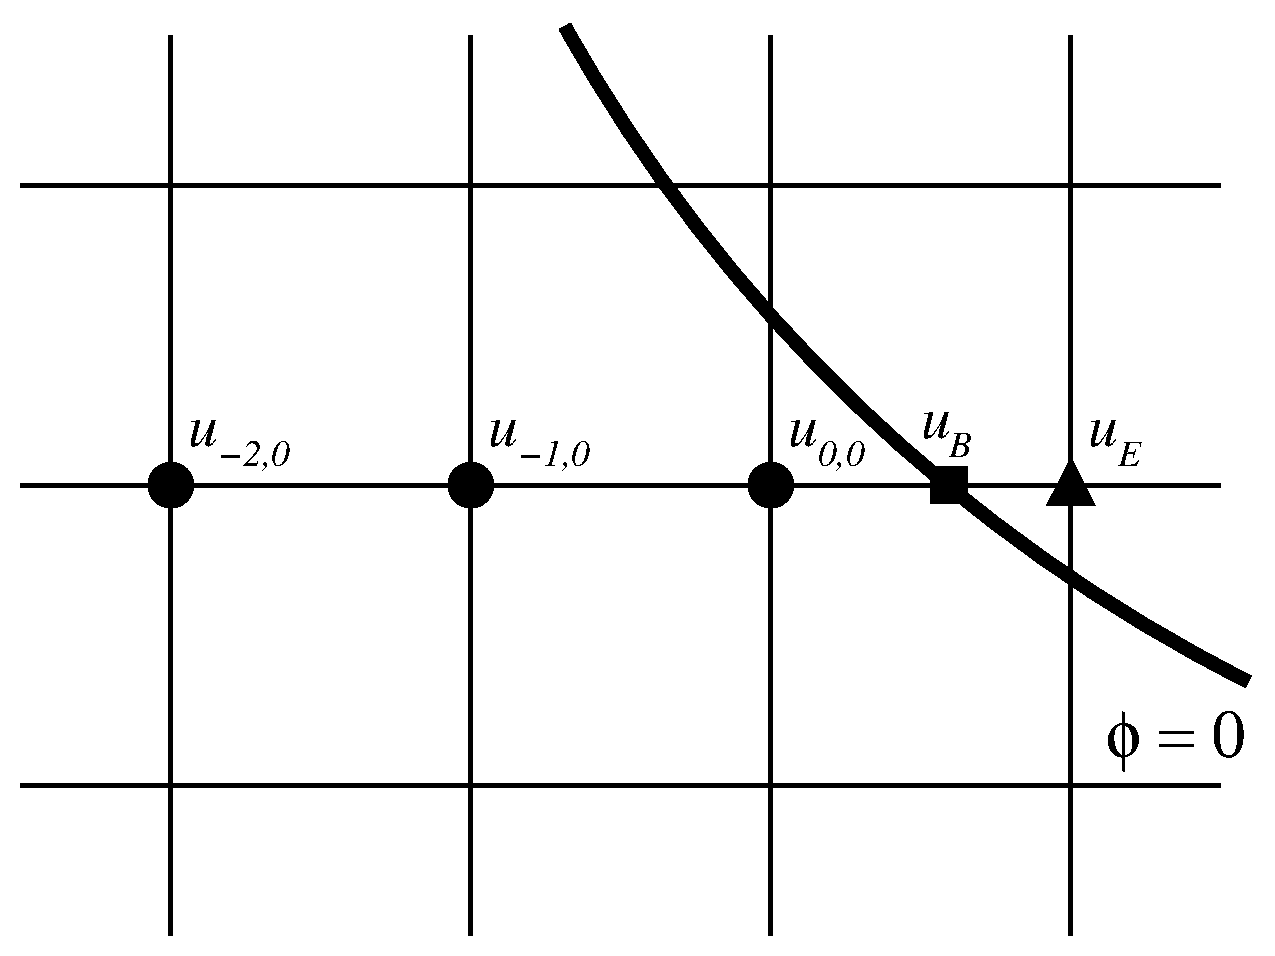
\includegraphics{figures/ghostcell_edge}} 
\ \ \ \ \ \ \ \ \ \ \ \ \ 
\scalebox{0.25}{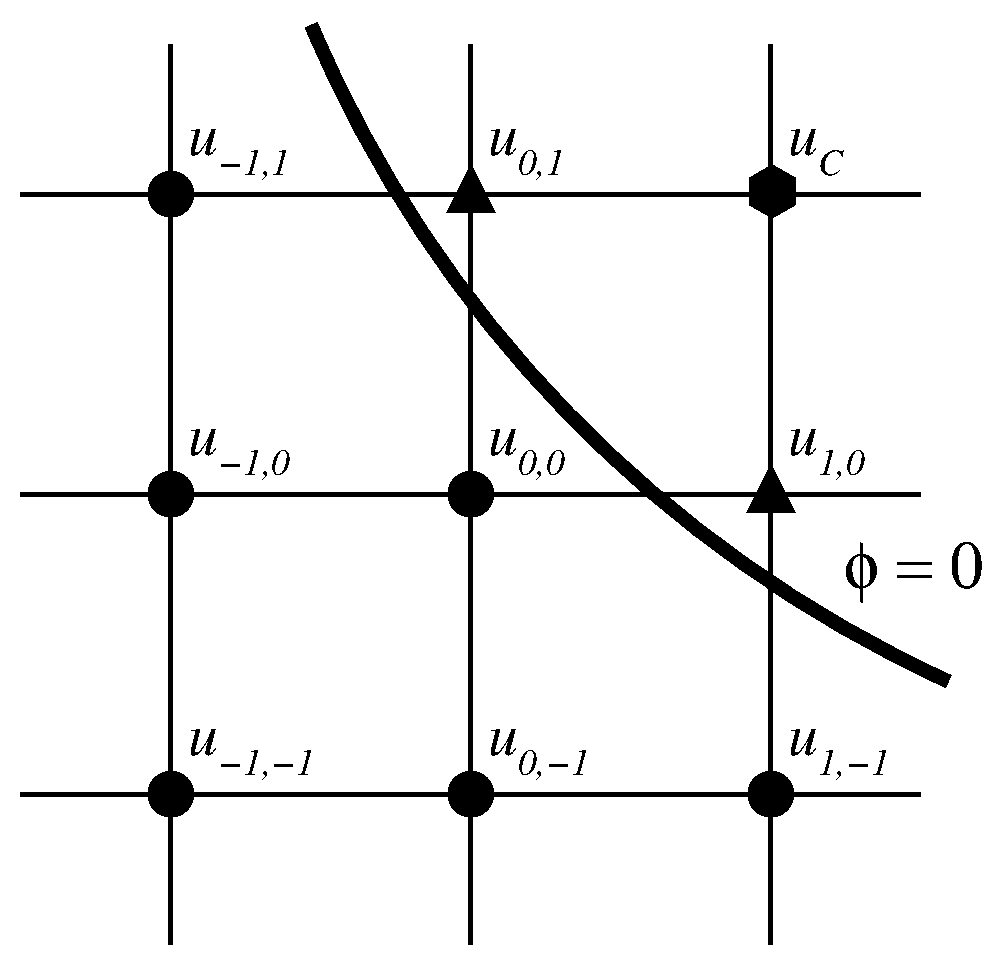
\includegraphics{figures/ghostcell_corner}}
\caption{Illustrations of edge (left) and corner (right) ghostcells.
The edge ghostcell, $u_E$, is filled by using cubic extrapolation of 
the value on the boundary, $u_B$, and values at three interior grid points.  
The corner ghostcell, $u_C$, is filled by using a fourth-order accurate
Taylor series expansion centered at $u_{0,0}$, which uses the values of $u$ 
at the specified interior grid points and neighboring edge ghost cells to 
approximate the partial derivatives in the expansion. 
}
\label{fig:ghost_cells}
\end{center}
\end{figure}

In this section, we extend the OTS finite difference scheme for the 2D 
diffusion equation on regular domains to irregular domains.  To avoid the 
need for special stencils at grid points near the irregular boundary, we adopt 
the `ghost cell' approach for imposing boundary conditions~\cite{gibou_2005, 
fedkiw_1999, osher_fedkiw_book}.  The basic idea is to set the value of $u$ at 
any grid point that lies immediately outside of the domain (and thus may be
required by spatial derivative operators at interior grid points) by 
extrapolating from values of $u$ at interior grid points and using boundary 
condition information.  
The main challenge is to find a method for filling ghost cells that does not 
decrease the accuracy of the solution in the interior of the domain.  For 
simplicity, we choose to represent the irregular boundary implicitly as the 
zero level set of a level set function $\phi$ which satisfies:
\bea
  \begin{array}{ll}
  \phi < 0 & \mathrm{for} \ x \in \Omega \\
  \phi > 0 & \mathrm{for} \ x \notin \Omega \\
  \phi = 0 & \mathrm{for} \ x \in \partial \Omega 
  \end{array}
\eea
where $\Omega$ and $\partial \Omega$ are the interior and boundary of the 
irregular domain.

Figure~\ref{fig:ghost_cells} shows examples of ghost cells that lie in the 
vicinity of an irregular boundary.  Notice that there are two types of ghost 
cells:  edge and corner.  Edge and corner ghost cells are distinguished by 
the relative position of the nearest interior grid point.  An edge ghost cell 
is linked to its nearest interior neighbor by an edge of the computational 
grid whereas a corner ghost cell and its nearest interior neighbor lie on the 
opposite corners of a grid cell.

To set the value of $u$ in each edge ghost cell, we use 1D, cubic 
extrapolation of the values of $u$ across the interface.  A cubic Lagrange 
interpolant is constructed for each edge ghost cell using a point on the 
domain boundary and three interior grid points that lie along the line 
parallel to the edge connecting the ghost cell to its nearest interior 
neighbor (see Figure~\ref{fig:ghost_cells}).  
The location of the point $u_B$ can be calculated by inverting the linear 
interpolant of $\phi$ that passes through the ghost cell and its nearest
interior neighbor\footnote{We found that using higher-order interpolants to 
locate boundary points was unnecessary for achieving high-order accuracy in 
the computed solution.}.  Because the quality of the interpolant deteriorates 
if the boundary point is too close to any of the interior grid points used to 
construct the Lagrange extrapolant, we follow \cite{gibou_2005} and choose the 
interior grid points so that the nearest interior grid point is sufficiently 
far from the boundary point.  Without this procedure, the errors introduced 
in the values of the ghost cells lead to instability of the numerical method.
Gibou~\etal~suggest shifting the interpolation points by one grid point 
when the distance between the boundary point and the nearest interior grid 
point is less than $\dx^2$~\cite{gibou_2005}.  For the numerical scheme 
presented in this paper, this threshold was too low.  We found that better 
stability was obtained if we used an $O(\dx)$ threshold.

% FIGURE SHOWING SOLUTION OF 2D DIFFUSION EQUATION ON STARFISH DOMAIN
% PLACED HERE TO SPREAD FIGURES OUT
\begin{figure}[tb]
\begin{center}
\scalebox{0.35}{\includegraphics{figures/diffusion_eqn_2d_starfish_domain_soln}} 
\scalebox{0.35}{\includegraphics{figures/diffusion_eqn_2d_starfish_domain_error}} 
\caption{Numerical solutions (left) and dominant error (right) for the 2D 
diffusion equation on a starfish-shaped domain.  The solution is computed at 
time $t = 0.1$ using forward Euler time stepping with an optimal time step 
and correction terms.  In the error plot, the dark regions represent points 
where the error in the solution is larger than $25$\% of the $L^\infty$ error 
of the solution.  For these figures, we use the same diffusion constant, 
source term, and initial conditions as described in the caption for 
Figure~\ref{fig:diffusion_eqn_2d_src_analysis}.  The boundary of the 
starfish-shaped domain is represented by the zero-level set of the function
$\sqrt{x^2 + y^2} - \frac{3}{5} \left(1 + \frac{1}{2}\sin(5 \theta) \right)$, 
where $\theta = \mathtt{atan}\left( y/x \right)$.
The Dirichlet boundary conditions are taken from the values of the analytical 
solution (see caption for Figure~\ref{fig:diffusion_eqn_2d_src_analysis})
on the irregular boundary.  The numerical solution is calculated using the 
square computational domain $-1 < x,y < 1$ which is discretized using 400 grid 
points in each coordinate direction (the plot of the solution has been 
downsampled for visualization purposes).  Boundary conditions are imposed by 
using fourth-order accurate approximations of the value of the solution in 
edge and corner ghost cells (described in the main text).
}
\label{fig:diffusion_eqn_2d_starfish_domain}
\end{center}
\end{figure}

To set the value of $u$ in a corner ghost cell, we use a fourth-order accurate
Taylor series expansion of $u$ centered at the nearest interior 
neighbor.  The partial derivatives in the Taylor series expansion are 
approximated using finite differences constructed from the values of $u$ 
at interior grid points and the neighboring edge ghost cells (see 
Figure~\ref{fig:ghost_cells}).  To obtain a fourth-order accurate value for 
the corner ghost cell, we need to carefully choose the finite difference 
stencils used for the partial derivatives.  For the corner ghost cell shown 
in Figure~\ref{fig:ghost_cells}, the extrapolation stencil is given by
\bea
  u_C &=&  -4 u_{0,0} - u_{-1,-1} + 2 u_{1,0} + 2 u_{0,1}
      - u_{1,-1} - u_{-1,1} + 2 u_{0,-1} + 2 u_{-1,0}
\eea
where $u_C$ and $u_{i,j}$ are indicated in the figure.  The stencils for
corner ghost cells that are in other positions relative to the interior of 
the domain are obtained by rotations of Figure~\ref{fig:ghost_cells} and 
remapping of the indicies in the above stencil.

Using these methods for filling edge and corner ghost cells, it is 
straightforward to compute high-order accurate solutions of the 2D diffusion 
equation on irregular domains.  We simply use the OTS forward Euler scheme 
designed for regular domains for grid points in the interior of the domain
after filling the ghost cells with high-order accurate values.  
Figure~\ref{fig:diffusion_eqn_2d_starfish_domain} shows an example of 
a solution computed on a starfish shaped domain.  It also shows that the 
error in the solution is concentrated near the boundaries of the irregular
domain.  Thus, we see that it is necessary to use high-order accurate 
extrapolants for the ghost cells to prevent errors at the boundary from 
destroying high-order accuracy throughout the domain.  The improved accuracy 
of the OTS solution compared to a simple forward Euler scheme with a 
suboptimal time step is illustrated in 
Figure~\ref{fig:diffusion_eqn_2d_starfish_error}. 

% FIGURE SHOWING SOLUTION OF 2D DIFFUSION EQUATION ON STARFISH DOMAIN
% PLACED HERE TO SPREAD FIGURES OUT
\begin{figure}[tb]
\begin{center}
\scalebox{0.35}{
  \includegraphics{figures/diffusion_eqn_2d_starfish_domain_error_vs_N}} 
\caption{$L^\infty$ error as a function of number of grid points for two
finite difference schemes that solve the 2D diffusion equation on an 
irregular domain: forward Euler with optimal time step and correction 
terms (circles) and forward Euler with suboptimal time step $\dt = \dx^2/4 D$
(squares).  Both methods solve the 2D diffusion equation described in the 
caption for Figure~\ref{fig:diffusion_eqn_2d_src_analysis} on the irregular
domain defined in the caption for 
Figure~\ref{fig:diffusion_eqn_2d_starfish_domain}.
These results were obtained using simple MATLAB implementations of the 
finite difference schemes.
}
\label{fig:diffusion_eqn_2d_starfish_error}
\end{center}
\end{figure}


\subsubsection{Diffusion Equation in Higher Dimensions}
Using optimal time step selection to boost the accuracy of finite difference
schemes for the diffusion equation in higher space dimensions is 
straightforward.  As for the 2D problem, the key step is identification of a 
finite difference stencil for the Laplacian that has an \emph{isotropic} 
discretization error.  For 3D problems, a catalog of several such stencils is 
available in~\cite{patra_2005}.   For higher dimensional problems, one simple
approach for deriving an isotropic finite difference stencil for the Laplacian
would be to start with the generalization of the standard five point stencil
for the 2D Laplacian and add finite difference approximations for the missing 
cross terms that are required to make the leading-order error isotropic 
(\ie proportional to the bilaplacian of the solution).  Because the missing 
terms are all of the form 
\beq
\frac{\dx^2}{6} \left(\frac{\partial^4 u}{\partial x_i^2 \partial x_j^2}\right),
\eeq
this approach is relatively easy to use.  To derive finite difference 
approximations with more general or complex properties, symbolic algebra 
software can be helpful~\cite{patra_2005, gupta_1998}.  

Once an acceptable finite difference approximation for the Laplacian has been 
chosen, the usual OTS analysis yields an optimal time step of 
$\dt_{opt} = \dx^2/6D$ for forward Euler time integration and a boost of the 
order of accuracy from two to four.  Above three dimensions, it is necessary 
to use an implicit time integration scheme because $\dt_{opt}$ is no longer 
stable for the forward Euler scheme.

Problems on irregular domains can be handled using the ghost cell approach. 
While the derivation of high accuracy stencils for ghost cells becomes more
tedious, the general approach is the same as for the 2D problem.  The ghost 
cells can first be grouped into separate classes based on the number of 
grid cell edges that must be traversed to reach the nearest interior neighbor.
The values in the ghost cells can then be set in order starting with those 
directly connected to their nearest interior neighbor and ending with those 
whose nearest interior neighbor is on the opposite corner of a grid cell.
Here, too, symbolic algebra programs can be helpful when deriving methods for 
extrapolating interior and boundary values to ghost cells.


\section{\label{sec:summary} Summary} 
In this paper, we have presented a novel approach for constructing high-order
finite difference methods for time dependent PDEs \emph{without} requiring
the use of high-order stencils or high-order time integration schemes.  
The basic idea is that the leading-order terms in the discretization error
can be eliminated by carefully choosing the time step and possibly adding
a few simple correction terms.  It is straightforward to derive both the 
optimal time step and the correction terms by (1) taking advantage of the 
regular structure of finite difference schemes and (2) making use of the
PDE to relate terms in the discretization error.  The boost in the order
of accuracy achieved when the optimal time step and correction terms is well
worth the extra effort required to explicitly retain and analyze the 
leading-order terms in the discretization error.   

Through many examples, we have demonstrated the utility of optimal time step
selection to a wide range of problems.  We showed how OTS selection can be 
used to very easily obtain high-order accurate solutions to many linear 
and semilinear PDEs in any number of space dimensions on both regular
and irregular domains.  The examples illustrate the surprisingly high-order
of accuracy that can be achieved using only low-order discretizations for 
spatial derivatives and simple forward Euler time integration.

Optimal time step selection is a simple example of the more general technique
of optimally selecting numerical parameters to boost the accuracy of 
numerical methods.  Little research appears to have been done in this area,
but, as OTS selection demonstrates, optimal selection of numerical parameters 
can significantly impact the accuracy of numerical methods.  To realize
the full potential of numerical methods, both optimal time step selection 
and optimal numerical parameter selection deserve further investigation.


% ACKNOWLEDGMENTS
\section*{Acknowledgments}
The author gratefully acknowledges the support of Vitamin D, Inc.
and the Institute for High-Performance Computing (IHPC) in Singapore. 
The author would like to thank P. Fok, M. Prodanovic, and A. Chiu for 
helpful suggestions on the manuscript.  The author particularly thanks P. Fok 
for many enlightening discussions. 

\bibliography{OTSPDE}

\end{document}
